\renewcommand{\prevlecture}{2 }
\renewcommand{\thislecture}{3 }
\renewcommand{\nextlecture}{4 }

%
% Cover page
%

\title[PHYS 201 / Lecture \thislecture]
{
  PHYS 201 / Lecture \thislecture\\
  {\it Electrical potential energy and potential, Circuital law,
       Poisson and Laplace equations, Boundary conditions, Uniqueness theorem}\\
}

\author[C.Andreopoulos] {
  Professor Costas Andreopoulos\inst{1,2}, {\it FHEA}
}
\institute[Liverpool/STFC-RAL] {
   \inst{1} University of Liverpool, Department of Physics\\
   \vspace{0.1cm}
   \inst{2} U.K. Research \& Innovation (UKRI), Science \& Technology Facilities Council,\\
            Rutherford Appleton Laboratory, Particle Physics Department\\
   \vspace{0.5cm}
   {\it {\color{magenta} Lectures delivered at the University of Liverpool, 2020-21}}\\
   \vspace{0.2cm}
}
\date{\today}

\titlegraphic{
  
\includegraphics[height=25px]{./images/logo/liverpool.png}
  \hspace{3px}
  
\includegraphics[height=30px]{./images/logo/ral.png}
}


\begin{frame}[plain]
  \titlepage
\end{frame}

% ------------------------------------------------------------------------------
% ------------------------------------------------------------------------------

%
% Revision of previous lecture
%

\renewcommand{\lecturesummarytitle}{Revision }
\renewcommand{\summarizedlecture}{2 }


%
%
%

\begin{frame}{Lecture \summarizedlecture - \lecturesummarytitle}

\begin{itemize}
{\small

\item {\bf Electric flux}
  \begin{itemize}
  {\small
     \item The electric flux $\Phi_E$ is the number of field lines of the electric field $\vec{E}$
           flowing through a surface S
        \begin{equation*}
          \Phi_E = \int_{S} \vec{E} d\vec{S}
        \end{equation*}
  }
  \end{itemize}

\item {\bf Gauss' law}
  \begin{itemize}
  {\small
     \item Our first Maxwell equation!
     \item In integral form (useful if a symmetry can be exploited to simplify the integral evaluation):
           Relates the flux through a closed surface with the net charge contained in it
           \begin{equation*}
              \int_{S} \vec{E} d\vec{S} = \frac{Q_{enc}}{\epsilon_0}
           \end{equation*}
     \item In differential form:
           Relates the divergence of the electric field with the local charge density
           \begin{equation*}
              \vec{\nabla} \vec{E} = \frac{\rho}{\epsilon_0}
           \end{equation*}
  }
  \end{itemize}

}
\end{itemize}

\end{frame}


%
% Plan for this lecture
%

\begin{frame}{Plan for Lecture \thislecture}

\begin{itemize}
  \item How much {\bf work} do I need to do {\bf to bring charges close together?}\\
    \vspace{0.2cm}
    We will calculate the work done to assemble
    \begin{itemize}
       \item discrete systems of 2, 3 and N charges, and
       \item a continuous distribution of charge characterised by density $\rho(\vec{r})$
    \end{itemize}
  \vspace{0.1cm}
  \item Will see that the work done is {\bf path-independent}.
  \vspace{0.1cm}
  \item Will explain that the work becomes the {\bf electric potential energy}
        of the system of charges and that it is stored in the electric field.
  \item Will introduce the concept of {\bf electric potential}.
  \vspace{0.1cm}
  \item Will study the {\bf circuital law} in differential and integral forms.
  \vspace{0.1cm}
  \item Will introduce the {\bf Poisson} and {\bf Laplace} equations.
  \vspace{0.1cm}
  \item In parallel, will continue revising some relevant maths:
    \begin{itemize}
      \item The Laplace operator, the "curl" of a vector field,
            boundary problems and the {\em uniqueness theorem}
    \end{itemize}
\end{itemize}
\end{frame}

% ------------------------------------------------------------------------------
% ------------------------------------------------------------------------------

%
%
%

\begin{frame}{Assembling a system of 2 same-sign charges}

Consider two same-sign charges separated by an infinite distance.\\
\vspace{0.2cm}
It is easy to understand that {\bf in order to bring the two charges closer together I need to do work.}\\
\vspace{0.3cm}

\begin{center}
  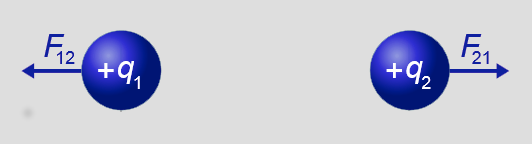
\includegraphics[width=0.70\textwidth]{./images/schematics/coulomb_force_2_like_sign_charges.png}\\
\end{center}

\vspace{0.2cm}
\underline{Why?}\\
\vspace{0.1cm}
Because {\bf they repel each other.} It is like pushing in a spring!

\end{frame}

% starting reminder
{
\reminderslide

%
%
%

\begin{frame}{Reminder: Work}

{\small

A force is said to {\bf do work} (denoted with W) if, when it is acting on a body,
there is a {\bf displacement of the point of application in the direction of the force}.
\vspace{0.3cm}

\begin{columns}
  \begin{column}{0.30\textwidth}
   \begin{center}
     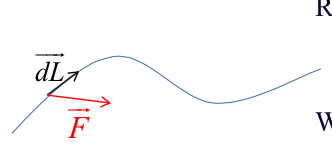
\includegraphics[width=0.99\textwidth]{./images/schematics/work.png}\\
   \end{center}
  \end{column}
  \begin{column}{0.70\textwidth}
    The work dW done by a force $\vec{F}$ displacing the point of application by $d\vec{\ell}$,
    is given by the dot product:
    \begin{equation*}
      dW = \vec{F} \cdot d\vec{\ell}
    \end{equation*}
    Notice that work is a {\bf scalar}.
    Its SI unit is a {\bf Joule (J)}: It is the work done by a force of 1 N over a distance of 1 m.
  \end{column}
\end{columns}

\vspace{0.3cm}
Note that {\bf a force perpendicular to the direction of motion does no work}.\\
\vspace{0.2cm}
The {\bf work can be positive or negative}.
By convention, we take work to be negative if it opposes the motion, i.e. $\theta > 90^{o}$.\\
\vspace{0.2cm}
The total work along a trajectory is given by integrating (summing up) the work done for
each infinitesimal displacement $d\vec{\ell}$: $W = \int dW = \int \vec{F} \cdot d\vec{\ell}$.\\
\vspace{0.2cm}
{\bf Work is very closely related to energy}.
}
\end{frame}

} % end reminder


%
%
%

\begin{frame}{Assembling a system of 2 same-sign charges}

We will answer the following question:
{\bf How much work is needed to bring 2 same-sign charges $q_1$ and $q_2$ from infinity to a distance $r_0$}?\\
\vspace{0.2cm}

\begin{columns}
  \begin{column}{0.70\textwidth}
   \begin{center}
     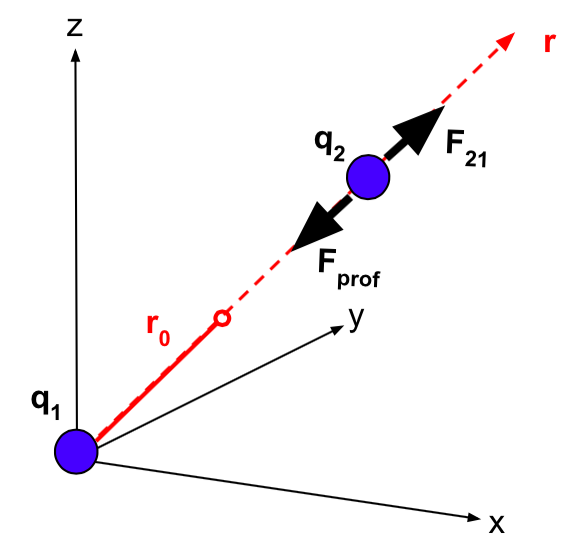
\includegraphics[width=0.80\textwidth]{./images/schematics/work_2_like_charges_2_q1q2.png}\\
   \end{center}
  \end{column}
  \begin{column}{0.30\textwidth}
   {\small
     \underline{Note}: \\
     \vspace{0.2cm}
     The two like charges repel each other.\\
     \vspace{0.2cm}
     I will calculate {\bf the work done by \underline{me} ($F_{prof}$)
     against the action of the field ($F_{21}$)},\\
     not the work done by the field force ($F_{21}$).\\
     \vspace{0.2cm}
     The difference between the two is a sign.\\
   }
  \end{column}
\end{columns}

\end{frame}

%
%
%

\begin{frame}{Work done assembling a system of 2 same-sign charges}

Placing charge $q_1$:\\

\begin{columns}
  \begin{column}{0.45\textwidth}
   \begin{center}
     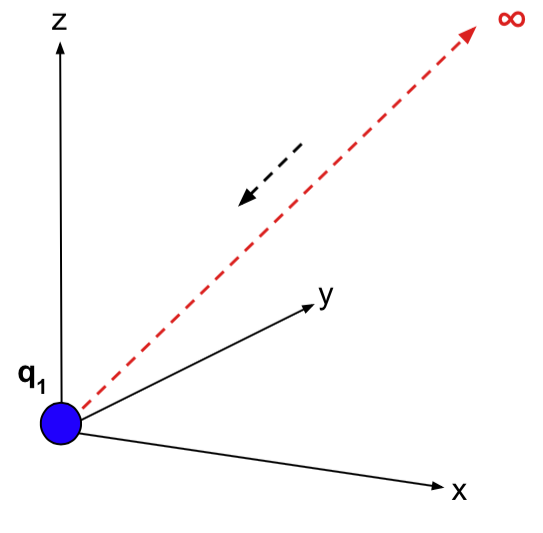
\includegraphics[width=0.99\textwidth]{./images/schematics/work_2_like_charges_2_q1.png}\\
   \end{center}
  \end{column}
  \begin{column}{0.54\textwidth}
   \begin{itemize}
   {\small
    \item Initially all charges are at {\em "infinity"}
       \begin{itemize}
       {\small
          \item i.e. far enough so that the force between them is so small that it can be neglected
       }
       \end{itemize}
    \vspace{0.2cm}
    \item I reach out all the way to infinity and grab charge $q_{1}$
    \vspace{0.2cm}
    \item I bring the charge $q_{1}$ at the origin of my coordinate system
       \begin{itemize}
       {\small
          \item There is no opposing force (other charges are still infinitely away)
       }
       \end{itemize}
    \vspace{0.2cm}
    \item That was an "easy" task
       \begin{itemize}
       {\small
         \item I did {\bf no work!}
       }
       \end{itemize}
   }
   \end{itemize}
  \end{column}
\end{columns}

\end{frame}


%
%
%

\begin{frame}{Work done assembling a system of 2 same-sign charges}

Placing charge $q_2$:\\

\begin{columns}
  \begin{column}{0.45\textwidth}
   \begin{center}
     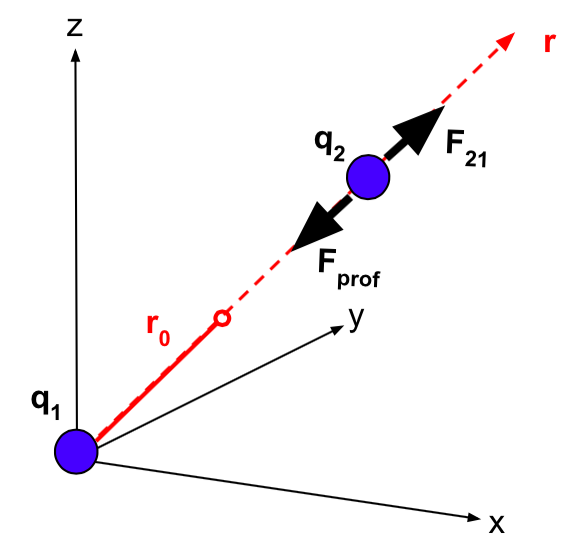
\includegraphics[width=0.99\textwidth]{./images/schematics/work_2_like_charges_2_q1q2.png}\\
   \end{center}
  \end{column}
  \begin{column}{0.55\textwidth}
   \begin{itemize}
   {\small
    \item I reach out all the way to infinity again and grab charge $q_2$ (same-sign as $q_1$).
    \item I begin to bring the charge $q_2$ closer to $q_1$, intending to pin it at $\vec{r_0}$.
    \vspace{0.2cm}
    \item There is an {\bf opposing force} due to $q_1$
    \item The force $\vec{F}_{21}$ exerted on charge $q_2$ due to charge $q_1$ is:
          \begin{equation*}
            \vec{F}_{21} = \frac{1}{4\pi\epsilon_0} \frac{q_1 q_2}{r^2} \hat{r}
          \end{equation*}
    \item I need to overcome this force so I apply a force $\vec{F}_{prof}$ which is:
          \begin{equation*}
            \vec{F}_{prof} = -\vec{F}_{21}
          \end{equation*}
   }
   \end{itemize}
  \end{column}
\end{columns}

\end{frame}


%
%
%

\begin{frame}{Work done assembling a system of 2 same-sign charges}

The {\bf work done by me} ($\vec{F}_{prof}$)
as I try {\bf to overcome the repulsive force} ($\vec{F}_{21}$) between $q_1$ and $q_2$
and move $q_2$  by an infinitesimally small distance $d\vec{\ell}$ is:
\begin{equation*}
  dW_{prof} =
    \vec{F}_{prof} \cdot d\vec{\ell} =
  - \vec{F}_{21} \cdot d\vec{\ell} =
  - \Big( \frac{1}{4\pi\epsilon_0} \frac{q_1 q_2}{r^2} \hat{r} \Big) \cdot d\vec{\ell}
\end{equation*}

The force is a radial vector. If I only move $q_2$ colinearly with  the force ($d\vec{\ell} = d\vec{r}$),
the above dot product simplifies to:
\begin{equation*}
  dW_{prof} = - \frac{q_1 q_2}{4\pi\epsilon_0} \frac{dr}{r^2}
\end{equation*}


The total work done to bring the $q_2$ from infinity to the position $\vec{r}_0$
is found by integrating $dW_{prof}$ from infinity ($\infty$) to $r_0$:
\begin{equation*}
  W_{prof} = \int_{\infty}^{r_{0}} dW_{prof} = - \frac{q_1 q_2}{4\pi\epsilon_0}  \int_{\infty}^{r_{0}}  \frac{dr}{r^2}
\end{equation*}

\end{frame}

%
%
%

\begin{frame}{Work done assembling a system of 2 same-sign charges}

I am sure that you can all calculate this integral:
\begin{equation*}
  W_{prof} = - \frac{q_1 q_2}{4\pi\epsilon_0}  \int_{\infty}^{r_{0}}  \frac{dr}{r^2}
\end{equation*}


The {\em anti-derivative} of $1/r^2$ is $-1/r$, so the integral becomes:

\begin{equation*}
\displaystyle
  W_{prof} = - \frac{q_1 q_2}{4\pi\epsilon_0} \Big( -\frac{1}{r} \Big)  {\rvert}_{\infty}^{r_{0}}
           = \frac{q_1 q_2}{4\pi\epsilon_0}  \Big( \frac{1}{r} \Big) {\rvert}_{\infty}^{r_{0}}
           = \frac{q_1 q_2}{4\pi\epsilon_0}  \Big( \frac{1}{r_0} - lim_{x\rightarrow\infty}\frac{1}{x} \Big) \Rightarrow
\end{equation*}
\begin{equation*}
  W_{prof} = \frac{q_1 q_2}{4\pi\epsilon_0 r_0}
\end{equation*}

\begin{blockminirem}{Mini reminder: Anti-derivatives}
 The {\em anti-derivative} of a function f is a differentiable function F whose derivative is equal to f (i.e. F$^{\prime}$ = f).
 Confirm that (-1/r)$^{\prime}$ = 1/r$^2$.
\end{blockminirem}

\end{frame}

%
%
%

\begin{frame}{Work done assembling a system of 2 \st{same-sign} charges}

We showed that the total work I need to do to assemble a system of 2 same-sign
charges $q_1$ and $q_2$ at distance $r_0$ is given by:
\begin{equation*}
  W_{prof} = \frac{q_1 q_2}{4\pi\epsilon_0 r_0}
\end{equation*}

The same result would have been obtained if, instead of considering 2 same-sign charges,
I had used one positive and one negative charge.\\

\vspace{0.2cm}

Notice that $W_{prof}$ involves the product $q_1 q_2$:

\begin{itemize}
   \item {\bf For same sign charges $q_1 q_2 > 0$}: \\
         To assemble that system I need to do {\bf positive work} (see convention discussed earlier).
         I need to spend energy because the force between the two charges is repulsive.
   \item {\bf For charges with different sign $q_1 q_2 < 0$}: \\
         To assemble that system I need to do {\bf negative work} as the force is attractive.
\end{itemize}

\end{frame}


%
%
%

\begin{frame}{Electrostatic potential energy of a system of 2 charges}

\vspace{0.1cm}
The work I did ($W_{prof}$) became the {\bf electrostatic potential energy of the system}
of two charges (usually denoted with U):
\begin{equation*}
  W_{prof} = U = \frac{q_1 q_2}{4\pi\epsilon_0 r_0}
\end{equation*}

\vspace{0.2cm}

\begin{itemize}
{
 \item
 The electrostatic potential energy is the energy of the system of $(q_1, q_2)$,
 {\bf not the energy of each of $q_1$ and $q_2$ individually}.\\

 \item
 As we shall see later in this course, this electrostatic potential energy is
 {\bf stored in the electric field} produced by the two charges.\\

 \item
 The potential energy (like the work done to assemble the system) can be positive or negative.
}
\end{itemize}

\end{frame}

%
%
%

\begin{frame}{Path-independence of work}

\begin{columns}
  \begin{column}{0.50\textwidth}
   \begin{center}
     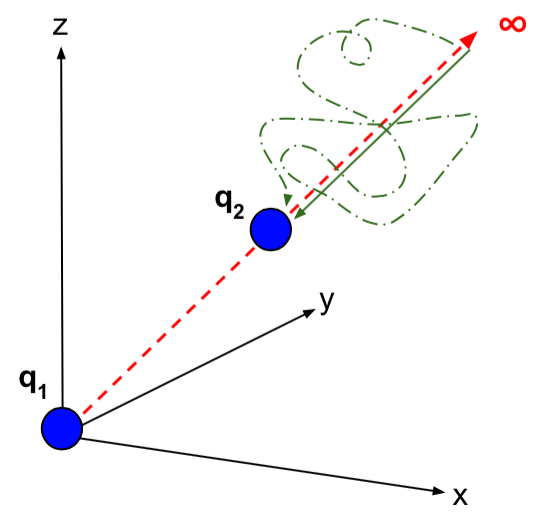
\includegraphics[width=0.99\textwidth]{./images/schematics/work_2_like_charges_2_q1q2_curved.png}\\
   \end{center}
  \end{column}
  \begin{column}{0.50\textwidth}
    We showed that the total work $W_{prof}$ that I need to do to assemble a system of 2 same-sign
    charges $q_1$ and $q_2$ at distance $r_0$, and hence the electrostatic potential energy U stored in the system,
    is given by:
    \begin{equation*}
      W_{prof} = U = \frac{q_1 q_2}{4\pi\epsilon_0 r_0}
    \end{equation*}
    I obtained that result by moving $q_2$ along a {\em straight} line that
    was collinear with the electric force.\\
  \end{column}
\end{columns}

\vspace{0.2cm}
There is an obvious question:\\
Would a {\bf longer curved trajectory give me a different result}?

\end{frame}

%
%
%

\begin{frame}{Path-independence of work}

The answer to the previous question is no.
\begin{itemize}
 \item The work done by the electric force is path-independent.\\
 \item We say then that {\bf the electric force is conservative}.\\
\end{itemize}

\vspace{0.3cm}

It is not difficult to understand that physically:
\begin{itemize}
{\small
 \item Work is converted to potential energy
       stored in the electric field.
 \item But identical charge configurations (given charges placed at given positions)
       produce the exact same field.
 \item Recall the general result for $\vec{E}$:
       \begin{equation*}
         \vec{E}(\vec{r}) = \frac{\vec{F}_{Q}}{Q} = \frac{1}{4\pi\epsilon_0} \int_{\tau}
            d\tau^{\prime} \frac{\rho({\pvec{r}'})}{|\vec{r}-\pvec{r}'|^{3}} (\vec{r}-\pvec{r}')
       \end{equation*}
       What matters is the distribution of charge, not how it got there.
 \item So the work done should be independent of the path.
}
\end{itemize}

\end{frame}

%
%
%

\begin{frame}{Path-independence of work}

{\small
We can show the path-independence mathematically.
It is sufficient to show this for charge moving {\bf between two infinitesimally separated spherical shells}.
%If it doesn't matter how I go from $\vec{r}$ to $\vec{r}+d\vec{r}$, then it doesn't matter how I go from $\vec{r}$ to any point.\\
}
\vspace{0.3cm}

\begin{columns}
  \begin{column}{0.50\textwidth}
   \begin{center}
     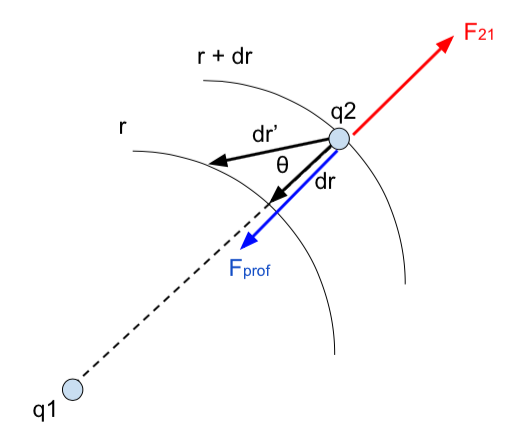
\includegraphics[width=0.88\textwidth]{./images/schematics/work_2_like_charges_2_q1q2_step.png}\\
   \end{center}
  \end{column}
  \begin{column}{0.50\textwidth}
  {\small
     The work done by moving $q_2$ along $d\vec{r}$ is:
     \begin{equation*}
       dW = \vec{F}_{prof} \cdot d\vec{r} = |\vec{F}_{prof}| |d\vec{r}|
     \end{equation*}
     whereas the work done by moving it along $d\pvec{r}'$ is:
     \begin{equation*}
       dW^{\prime} = \vec{F}_{prof} \cdot d\pvec{r}' = |\vec{F}_{prof}| |d\pvec{r}'| cos\theta
     \end{equation*}
     But $|d\vec{r}| = |d\pvec{r}'| cos\theta$, therefore:
     \begin{equation*}
       dW = dW^{\prime}
     \end{equation*}
  }
  \end{column}
\end{columns}

\vspace{0.1cm}
{\small
Hint: Since the result is path-independent, choose a path that simplifies the calculations
(usually, by exploiting the symmetries of the problem)
}

\end{frame}

%
%
%

\begin{frame}{Generalisation for 3 charges}

How about a slightly more complex system that has 3 charges $q_1$, $q_2$, $q_3$?\\
\vspace{0.2cm}

\begin{columns}
  \begin{column}{0.60\textwidth}
   \begin{center}
     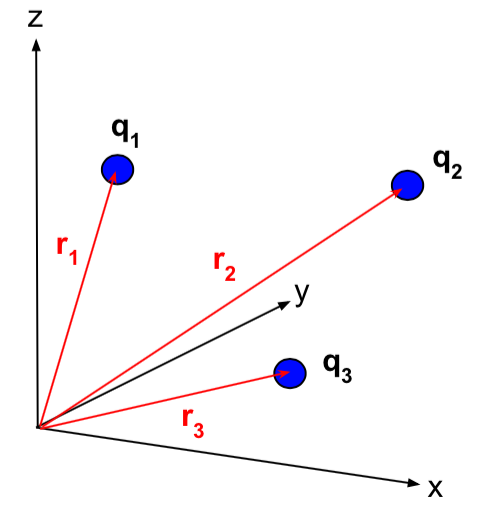
\includegraphics[width=0.85\textwidth]{./images/schematics/work_3_charges.png}\\
   \end{center}
  \end{column}
  \begin{column}{0.40\textwidth}
     The question now becomes:\\
     \vspace{0.3cm}
     {\bf How much work is needed to assemble}
     (or, how much potential energy is stored in)
     {\bf a system of 3 charges?}\\
  \end{column}
\end{columns}

\end{frame}

%
%
%

\begin{frame}{Generalisation for 3 charges}

\begin{itemize}

  \item To assemble a system of 3 charges, I need to add a charge $q_3$ to a system of 2 charges $q_1$ and $q_2$.

  \vspace{0.2cm}
  \item We already know how much work is needed to bring the first 2 charges together
        or, equivalently, what is the electrostatic potential energy stored in this system.

  \vspace{0.2cm}
  \item If $q_1$ is brought at position $\vec{r}_1$ and $q_2$ at position $\vec{r}_2$,
        the energy stored in the system is:
        \begin{equation*}
           U = \frac{q_1 q_2}{4\pi\epsilon_0 |\vec{r}_{12}|}
        \end{equation*}
        where $|\vec{r}_{12}| = |\vec{r}_1 - \vec{r}_2|$ is the distance between $q_1$ and $q_2$.\\
        \vspace{0.2cm}
        {\it (Here, I changed the notation slightly ($r_0 \rightarrow |\vec{r}_{12}|$)
        to help me generalise the result obtained previously for 2 charges.)}
\end{itemize}

\end{frame}

%
%
%

\begin{frame}{Generalisation for 3 charges}

So, the problem is reduced to finding out {\bf how much work is needed
to add the charge $q_3$ to the system of $q_1$ and $q_2$}.\\
\vspace{0.2cm}

The superposition principle applies
(the total force on a charge due to an array of other charges is the vector sum of the individual forces):
\begin{equation*}
  \vec{F} = \sum_{i} \vec{F}_{i}
\end{equation*}
So, the total field force $\vec{F}_{3}$ exerted on $q_3$ is:
\begin{equation*}
  \vec{F}_{3} = \vec{F}_{31} + \vec{F}_{32}
\end{equation*}
where $\vec{F}_{31}$ ($\vec{F}_{32}$) is the force exerted on $q_3$ due to $q_1$ ($q_2$).\\

\end{frame}

%
%
%

\begin{frame}{Generalisation for 3 charges}

\vspace{0.2cm}
Therefore, the work that I need to do against the action of the field (i.e. against $\vec{F}_{3}$) is:
\begin{equation*}
  W_{prof} = \int \vec{F}_{prof} \cdot d\vec{\ell}
           = - \int \vec{F}_{3} \cdot d\vec{\ell}
           = - \int \vec{F}_{31} \cdot d\vec{\ell} - \int \vec{F}_{32} \cdot d\vec{\ell} \Rightarrow
\end{equation*}

\begin{equation*}
  W_{prof} = W_{prof;1} + W_{prof;2}
\end{equation*}

\vspace{0.3cm}
What this tells us is that, in order to bring $q_3$ at position $\vec{r}_3$,
after $q_1$ was brought at position $\vec{r}_1$ and $q_2$ at $\vec{r}_2$,
I need to do work which is the sum of:\\
\vspace{0.1cm}
\begin{itemize}
  \item the work I would need to do if only $q_1$ was in place, and
  \item the work I would need to do if only $q_2$ was in place.
\end{itemize}

{\bf My 3-charge problem is reduced to a number of 2-charge problems} (for which I know the solutions).

\end{frame}


%
%
%

\begin{frame}{Generalisation for 3 charges}

So the previous observation allows us to calculate the work
(or total potential energy) {\bf by considering all possible sub-systems of 2 charges}.\\

\begin{columns}
  \begin{column}{0.55\textwidth}
   \begin{center}
     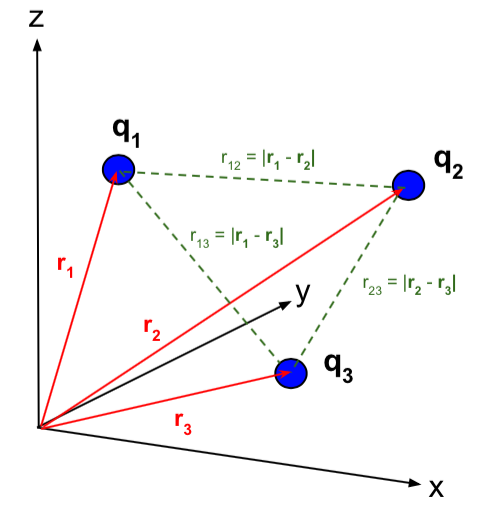
\includegraphics[width=0.95\textwidth]{./images/schematics/work_3_charges_with_distances.png}\\
   \end{center}
  \end{column}
  \begin{column}{0.45\textwidth}
     How many distinct sub-systems of 2 charges are there in the system of 3 charges?\\
     \vspace{0.3cm}
     The obvious answer is 3:
     \begin{itemize}
     {
        \item ($q_1$, $q_2$) separated by distance $|\vec{r}_{12}|$,
        \item ($q_1$, $q_3$) separated by distance $|\vec{r}_{13}|$, and
        \item ($q_2$, $q_3$) separated by distance $|\vec{r}_{23}|$.\\
     }
     \end{itemize}
  \end{column}
\end{columns}

\end{frame}

%
%
%

\begin{frame}{Generalisation for 3 charges}

Therefore, the work I need to do to assemble
(and, consequently the total potential energy stored in)
the system of 3 charges is:
\begin{equation*}
  U = \frac{q_1 q_2}{4\pi\epsilon_0 |\vec{r}_{12}|} +
      \frac{q_1 q_3}{4\pi\epsilon_0 |\vec{r}_{13}|} +
      \frac{q_2 q_3}{4\pi\epsilon_0 |\vec{r}_{23}|}
\end{equation*}

Here, I made no assumption about the charge signs:
\begin{itemize}
{\small
   \item They can be anything, in any combination (+++, ++-, +-+, -++, ...)
   \item For some of the pairs above I may need to do positive work, while for others I may need to do negative work.
   \item The total work I need to do is the algebraic sum.
   \item The total work may have either sign, depending on which terms dominate.
}
\end{itemize}

\vspace{0.4cm}
{\bf What to remember}: \\
My 3-charge problem was reduced to a number of 2-charge problems. \\
Each pair contributes a $\frac{q_i q_j}{4\pi \epsilon_0 |\vec{r}_{ij}|}$ term to the total potential energy.\\

\end{frame}

%
%
%

\begin{frame}{Generalisation for N charges}

We can generalise our result for a {\bf system of N charges $q_1$, $q_2$, $q_3$,..., $q_N$}.\\
\vspace{0.2cm}

There is a clear recipe for calculating the total potential energy:
\begin{itemize}
  \item Find all distinct pairs of charges.
  \item Every distinct pair will contribute with a $\frac{q_i q_j}{4\pi \epsilon_0 |\vec{r}_{ij}|}$ term.\\
\end{itemize}
\vspace{0.2cm}

Therefore the total potential energy can be written as:
\begin{equation*}
  U = {\color{red} \sum_{all\; pairs}} \frac{q_i q_j}{4\pi \epsilon_0 |\vec{r}_{ij}|}
\end{equation*}

\vspace{0.2cm}
The question now becomes {\bf how to enumerate all possible pairs}.

\end{frame}

\vspace{0.2cm}

%
%
%

\begin{frame}{Generalisation for N charges}

{\bf How many pairs are there in the system of N charges?} \\
\vspace{0.2cm}

The number of groups of $k$ items we can select from a collection of $n$ items ($k<=n$),
if the order of the selection does not matter, is given by the {\bf Binomial Coefficient}:

\begin{equation*}
  \left(
    \begin{array}{c}
      n \\
      k
    \end{array}
  \right) =
  \frac{n!}{k!(n-k)!} =
  \frac{n(n-1)...(n-k+1)}{k(k-1)...1}
\end{equation*}

For example:

\begin{itemize}
  \item for N = 4 charges, the numbers of pairs is
        $\left(
          \begin{array}{c}
            4 \\
            2
          \end{array}
        \right) = 6$
  \item for N = 10 charges, the numbers of pairs is
        $\left(
          \begin{array}{c}
           10 \\
            2
          \end{array}
        \right) = 45$
\end{itemize}

We need a way to take all pairs into account systematically
{\bf so that we do not neglect or double-count terms}.

\end{frame}

%
%
%

\begin{frame}{Generalisation for N charges}

Let's think about {\bf a systematic procedure for forming pairs}:\\
\vspace{0.2cm}

\begin{itemize}
  \item We {\bf start with charge $q_1$} and we pair it with all charges.\\
        \vspace{0.2cm}
        The pairs are {\color{red}($\cancel{q_1,q_1}$), ($q_1,q_2$), ($q_1,q_3$),..., ($q_1,q_N$)}.\\
        \vspace{0.2cm}
        \begin{itemize}
           \item We do not include "self-energy" terms
                 (i.e. we don't consider the terms obtained by pairing each charge with "itself")
                 so we neglect ($q_1,q_1$).
        \end{itemize}
  \vspace{0.3cm}
  \item Let's {\bf move to charge $q_2$} and pair it with all charges.\\
        \vspace{0.2cm}
        The new pairs are {\color{red}($\cancel{q_2,q_1}$),($\cancel{q_2,q_2}$),($q_2,q_3$),...,($q_2,q_N$)}.
        \vspace{0.2cm}
        \begin{itemize}
           \item As before, we don't include the self-energy term ($q_2,q_2$).
           \item But we also neglect ($q_2,q_1$). This is the same as  ($q_1,q_2$) that was already taken into account.
        \end{itemize}
\end{itemize}

\vspace{0.3cm}
You probably start to see the pattern here.

\end{frame}

%
%
%

\begin{frame}{Generalisation for N charges}

To take into account all distinct pairs, we sum over the charges $q_i$ and, for each $q_i$,
we sum over the charges $q_j$ but with j starting from i+1 (not from 1):
\begin{equation*}
     U = {\color{red} \sum_{i=1} \sum_{j=i+1} } \frac{q_i q_j}{4\pi\epsilon_0 |\vec{r}_{ij}|}
\end{equation*}

\vspace{0.2cm}

We need to be {\bf careful towards the end of the double sum}:
\begin{itemize}
     \item If i=N-1 (the last but one charge), then there is only one pair
           left to be formed with j=N: {\color{red} ($q_{N-1}$, $q_N$)}.
     \item So my double sum {\bf ends when i=N-1 and j=N}.
\end{itemize}

\vspace{0.2cm}

Therefore, the expression for the total potential energy of a system of N charges becomes:
\begin{equation*}
   U = {\color{red}\sum_{i=1}^{N-1} \sum_{j=i+1}^{N}} \frac{q_i q_j}{4\pi\epsilon_0|\vec{r}_{ij}|}
\end{equation*}

\end{frame}

%
%
%

\begin{frame}{Generalisation for N charges}

The table below shows all $q_{i}q_{j}$ terms we included (\ck).
We {\bf can re-write the sum in a more symmetric way}.

\begin{columns}
  \begin{column}{0.63\textwidth}
   \begin{center}
    {\scriptsize
    \begin{table}
    \begin{tabular}{|c|c|c|c|c|c|c|c|c|c|}
      \hline
           &           & \multicolumn{8}{c|}{\bf j}\\
           &           & $q_1$ & $q_2$ & $q_3$ & $q_4$ & $q_5$ & ... & $q_{N-1}$ & $q_N$   \\
      \hline
       \multirow{8}{*}{\bf i}
           & $q_1$     & -     & \ck   & \ck   & \ck   & \ck   & ... & \ck   & \ck     \\
           & $q_2$     & -     & -     & \ck   & \ck   & \ck   & ... & \ck   & \ck     \\
           & $q_3$     & -     & -     & -     & \ck   & \ck   & ... & \ck   & \ck     \\
           & $q_4$     & -     & -     & -     & -     & \ck   & ... & \ck   & \ck     \\
           & $q_5$     & -     & -     & -     & -     & -     & ... & \ck   & \ck     \\
           & ...       & ...   & ...   & ...   & ...   & ...   & ... & ...   & ...     \\
           & ...       & ...   & ...   & ...   & ...   & ...   & ... & ...   & ...     \\
           & $q_{N-1}$ & -     & -     & -     & -     & -     & ... & -     & \ck     \\
           & $q_N$     & -     & -     & -     & -     & -     & ... & -     & -       \\
      \hline
    \end{tabular}
    \end{table}
   }
   \end{center}
  \end{column}
  \begin{column}{0.37\textwidth}
     \begin{itemize}
     {\small
        \item What happens if I just sum up over all charges, without the $j>i$ condition,
              excluding only the self-terms?
        \item Obviously, I {\bf count each pair twice}:
              E.g, I consider both {\color{red}($q_1,q_2$)} and {\color{red}($q_2,q_1$)}.
     }
     \end{itemize}
  \end{column}
\end{columns}

\vspace{0.2cm}
So I can just rewrite the sum as:
     \begin{equation*}
        U = \sum_{i=1}^{N-1} \sum_{j=i+1}^{N} \frac{q_i q_j}{4\pi\epsilon_0|\vec{r}_{ij}|} {\color{blue} \;\; \rightarrow \;\;}
        {\color{red} \frac{1}{2}} \sum_{{\color{red}i,j=1;i{\ne}j}}^{N} \frac{q_i q_j} {4\pi\epsilon_0|\vec{r}_{ij}|}
     \end{equation*}

\end{frame}


%
%
%

\begin{frame}{Generalisation for continuous charge distributions}

We will now make the {\bf leap from discrete to continuous distributions of charge}
characterised by a volume charge density $\rho(\vec{r})$.

\begin{columns}
  \begin{column}{0.50\textwidth}
   \begin{center}
     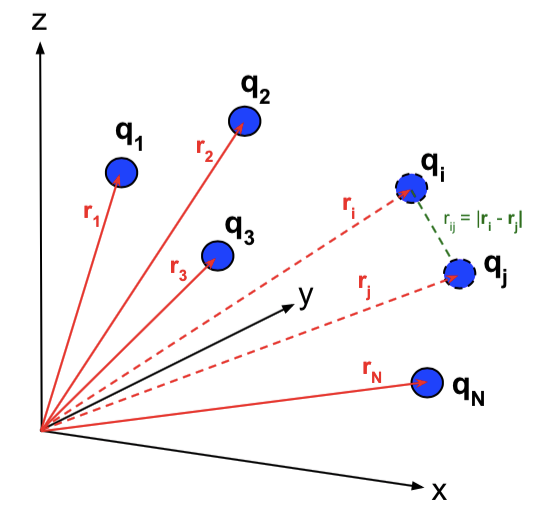
\includegraphics[width=0.95\textwidth]{./images/schematics/work_n_charges.png}\\
   \end{center}
  \end{column}
  \begin{column}{0.50\textwidth}
   \begin{center}
     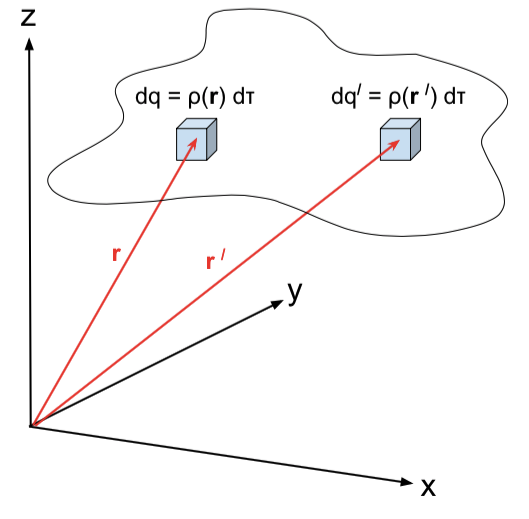
\includegraphics[width=0.95\textwidth]{./images/schematics/work_continuous_distribution.png}\\
   \end{center}
  \end{column}
\end{columns}

\end{frame}


%
%
%

\begin{frame}{Generalisation for continuous charge distributions}

Our starting point, is the result obtained for N charges:
\begin{equation*}
   U = \frac{1}{2} \sum_{i,j=1;i{\ne}j}^{N} \frac{q_i q_j}{4\pi\epsilon_0|\vec{r}_{ij}|}
\end{equation*}

%If $\rho(\vec{r})$ is the amount of charge per unit volume, the amount of charge contained
%within a small volume $d\tau$ around the position $\vec{r}$ is $\rho(\vec{r}) d\tau$.

This result can be readily adapted for the continuous case
by making the following substitutions:

\begin{itemize}
   \item $q_{i} \rightarrow dq(\vec{r}) = \rho(\vec{r}) d\tau$
   \item $q_{j} \rightarrow dq(\vec{r^{\prime}}) = \rho(\vec{r^{\prime}}) d\tau^{\prime}$
   \item $|\vec{r}_{ij}| \rightarrow |\vec{r} - \vec{r^{\prime}}|$
   \item $\sum \rightarrow \int$
\end{itemize}

The electrostatic potential energy for a continuous charge distribution characterised
by density $\rho$ can be written as:
\begin{equation*}
    U = \frac{1}{2} \int_{vol} d\tau \int_{vol} d\tau^{\prime}
          \frac{\rho(\vec{r}) \rho(\vec{r^{\prime}})}{4\pi\epsilon_0|\vec{r} - \vec{r^{\prime}}|}
\end{equation*}

\end{frame}


%
%
%

\begin{frame}{Summary of basic results}

Potential energy stored in a:

\begin{itemize}
\item {\bf system of 2 charges}:
 \begin{equation*}
   U = \frac{q_1 q_2}{4\pi\epsilon_0} \frac{1}{|\vec{r}_{12}|}
 \end{equation*}

\item {\bf system of 3 charges}:
 \begin{equation*}
   U = \frac{q_1 q_2}{4\pi\epsilon_0} \frac{1}{|\vec{r}_{12}|} +
       \frac{q_1 q_3}{4\pi\epsilon_0} \frac{1}{|\vec{r}_{13}|} +
       \frac{q_2 q_3}{4\pi\epsilon_0} \frac{1}{|\vec{r}_{23}|}
 \end{equation*}

\item {\bf system of N charges}:
 \begin{equation*}
   U = \frac{1}{2} \sum_{i,j=1;i{\ne}j}^{N} \frac{q_i q_j}{4\pi\epsilon_0|\vec{r}_{ij}|}
 \end{equation*}

\item {\bf continuous charge distribution} (with density $\rho$ over a volume $\tau$):
 \begin{equation*}
    U = \frac{1}{2} \int_{vol} d\tau \int_{vol} d\tau^{\prime}
        \frac{\rho(\vec{r}) \rho(\vec{r^{\prime}})}{4\pi\epsilon_0|\vec{r} - \vec{r^{\prime}}|}
 \end{equation*}

\end{itemize}
\end{frame}


% ------------------------------------------------------------------------------

%
% Worked example
%

{
\problemslide

%
%
%

\begin{frame}{Worked example: Potential of 4 charges on square }

\begin{blockexmplque}{Question}
\begin{columns}
  \begin{column}{0.25\textwidth}
   \begin{center}
     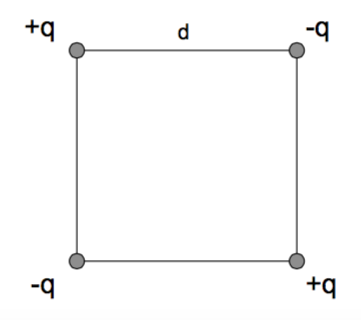
\includegraphics[width=0.98\textwidth]{./images/problems/lect2_array_of_4_charges.png}
   \end{center}
  \end{column}
  \begin{column}{0.75\textwidth}
     Four charges each of magnitude q are located at the four corners of a
     square of side d such that like charges occupy the corners across
     the diagonals. \\
    Calculate the work done in assembling these charges.
  \end{column}
\end{columns}
\end{blockexmplque}

\vspace{0.1cm}

Work done is
$\displaystyle W = U_{12} + U_{23} + U_{34} + U_{41} + U_{13} + U_{24}$
where $\displaystyle U_{ij} =  \frac{q_i q_j}{4\pi \epsilon_0 r_{ij}}$

Numbering charges clock-wisely from top left one,
so that charges 1 and 3 are positive and 2 and 4 negative:
\begin{equation*}
  W = \frac{1}{4\pi \epsilon_0}
    \bigg\{
        - \frac{q^2}{d} -  \frac{q^2}{d} -  \frac{q^2}{d} -  \frac{q^2}{d} +  \frac{q^2}{\sqrt{2}d} + \frac{q^2}{\sqrt{2}d}
     \bigg\} =
     -\frac{q^2}{4\pi \epsilon_0 d} \Big( 4 - \sqrt{2} \Big)
\end{equation*}

\end{frame}

} % Example

% ------------------------------------------------------------------------------

%
% Worked example
%

{
\problemslide

\begin{frame}{Worked example: Potential of 3 charges on a line }

\begin{blockexmplque}{Question}
    Two particles of charges $q_1$ and $q_2$ are fixed to an x axis,
  	as shown below.
    If a third particle, of charge +6.0 $\mu$C, is brought from an infinite
  	distance to point P, the three-particle system has the same electric
  	potential energy as the original two-particle system.
  	What is the charge ratio $q_2$/$q_1$?
    \begin{center}
      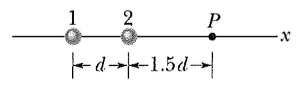
\includegraphics[width=0.50\textwidth]{./images/problems/lect03_2_point_charges}
    \end{center}
\end{blockexmplque}

\end{frame}

%
%
%

\begin{frame}{Worked example: Potential of 3 charges in line }

By adding a particle with charge q at point P,
at a distance $r_1$ from $q_1$ and at distance $r_2$ from $q_2$,
the change in the electrostatic potential
energy of the system is given by:
\begin{equation*}
  	{\Delta}U = \frac{q_1 q}{4\pi\epsilon_0 r_1} + \frac{q_2 q}{4\pi\epsilon_0 r_2}
\end{equation*}

Since ${\Delta}U$ = 0, we have:
\begin{equation*}
	\frac{q_1 q}{4\pi\epsilon_0 r_1} + \frac{q_2 q}{4\pi\epsilon_0 r_2} = 0 \Rightarrow
\end{equation*}
\begin{equation*}
	\frac{q_1}{r_1} + \frac{q_2}{r_2} = 0 \xRightarrow{r_1=2.5d,\;r_2=1.5d}
	\frac{q_1}{2.5} + \frac{q_2}{1.5} = 0 \Rightarrow
\end{equation*}
\begin{equation*}
	\frac{q_2}{q_1} = -\frac{1.5}{2.5} = -\frac{3}{5} = -0.6
\end{equation*}

\end{frame}

} % Example

% ------------------------------------------------------------------------------

%
%
%

\begin{frame}{Force and potential energy}

Earlier, we saw that
\begin{equation*}
  U = \int \vec{F} \cdot d\vec{\ell}
\end{equation*}

So {\bf given a force} (on all points along our trajectory)
{\bf we can calculate} the work done and thus {\bf the electrostatic potential energy}.\\

\vspace{0.3cm}

But what if we wanted to solve the opposite problem?\\
Suppose that, somehow, we knew the potential energy for adding a charge anywhere on space
and we wanted to calculate the force on that charge?\\

\vspace{0.2cm}

This would require {\em inverting} the above equation.\\

\vspace{0.2cm}

As you have also seen in mechanics,
we can express the force in terms of the gradient of U:
\begin{equation*}
  \vec{F} = -\vec{\nabla}U
\end{equation*}

\end{frame}

%
% Worked example
%

{
\problemslide

%
%
%

\begin{frame}{Worked example: Finding $\vec{F}$ from U}

\begin{blockexmplque}{Question}
Starting from the Coulomb force between two charges Q and q,
we estimated the following potential energy U for the system of two charges:
\begin{equation*}
  U = \frac{Qq}{4\pi\epsilon_0 |\vec{r}|}
\end{equation*}
where $|\vec{r}| = \sqrt{x^2 + y^2 + z^2}$.
Can you derive the Coulomb force between charges Q and q
starting from the above potential energy U?
\end{blockexmplque}

The force is given by:
\begin{equation*}
  \vec{F} = -\vec{\nabla}U
\end{equation*}

The gradient of U is:
\begin{equation*}
  \vec{\nabla}U =
     \Big(
       \frac{\partial U}{\partial x},
       \frac{\partial U}{\partial y},
       \frac{\partial U}{\partial z}
     \Big) =
     \frac{\partial U}{\partial x} \hat{x} +
     \frac{\partial U}{\partial y} \hat{y} +
     \frac{\partial U}{\partial z} \hat{z}
\end{equation*}

\end{frame}

%
%
%

\begin{frame}{Worked example: Finding $\vec{F}$ from U}

Substituting U from we have:
\begin{equation*}
  \vec{\nabla}U =
     \frac{Qq}{4 \pi \epsilon_0}
     \Big(
       \frac{\partial}{\partial x},
       \frac{\partial}{\partial y},
       \frac{\partial}{\partial z}
     \Big) \frac{1}{|\vec{r}|}
\end{equation*}

The partial derivative $\frac{\partial}{\partial x} \frac{1}{|\vec{r}|}$ is calculated as follows:

\begin{equation*}
  \frac{\partial}{\partial x} \frac{1}{|\vec{r}|} =
  \frac{\partial}{\partial x} \frac{1}{\sqrt{x^2 + y^2 + z^2}} =
  \frac{\partial}{\partial x} \Big( x^2 + y^2 + z^2 \Big) ^{-\frac{1}{2}} =
\end{equation*}

\begin{equation*}
   = -\frac{1}{2} \Big( x^2 + y^2 + z^2 \Big) ^{-\frac{3}{2}} (2x) =
   \frac{-x}{\Big( \sqrt{x^2 + y^2 + z^2} \Big)^{3}} =
   \frac{-x}{|\vec{r}|^3}
\end{equation*}

Similarly:

\begin{equation*}
  \frac{\partial}{\partial y} \frac{1}{|\vec{r}|} = \frac{-y}{|\vec{r}|^3}
  \;\;\;\;\; and \;\;\;\;\;
  \frac{\partial}{\partial z} \frac{1}{|\vec{r}|} = \frac{-z}{|\vec{r}|^3}
\end{equation*}

\end{frame}

%
%
%

\begin{frame}{Worked example: Finding $\vec{F}$ from U}

Therefore:
\begin{equation*}
  \vec{\nabla}U =
     \frac{Qq}{4 \pi \epsilon_0}
     \Big(
       \frac{\partial}{\partial x},
       \frac{\partial}{\partial y},
       \frac{\partial}{\partial z}
     \Big) \frac{1}{|\vec{r}|} =
     \frac{Qq}{4 \pi \epsilon_0}
     \Big(
       \frac{-x}{|\vec{r}|^3},
       \frac{-y}{|\vec{r}|^3},
       \frac{-z}{|\vec{r}|^3}
     \Big) =
     - \frac{Qq}{4 \pi \epsilon_0} \frac{\vec{r}}{|\vec{r}|^3}
\end{equation*}

Since $\vec{F} = -\vec{\nabla}U$
the force $\vec{F}$ is given by:
\begin{equation*}
  \vec{F} = \frac{Qq}{4 \pi \epsilon_0} \frac{\vec{r}}{|\vec{r}|^3}
\end{equation*}

This is our well-known Coulomb force between charges Q and q.\\
\vspace{0.1cm}

\noindent\rule{2cm}{0.4pt}\\
{\scriptsize
Note: Since the potential energy has only radial dependence,
the above calculation could be simplified by using the gradient in spherical coordinates:

\begin{equation*}
  \vec{\nabla}U =
     \frac{\partial U}{\partial r} \hat{r} +
     \frac{1}{r} \frac{\partial U}{\partial \theta} \hat{\theta} +
     \frac{1}{r sin\theta} \frac{\partial U}{\partial \phi} \hat{\phi}
\end{equation*}

Try this on your own.
}

\end{frame}

} % Example


%
%
%

\begin{frame}{Circuital law for Electrostatics}

As we saw earlier, the work $W = \int \vec{F} \cdot d\vec{\ell}$
done to move a charge from point a to b is independent of the path followed between a and b.\\
\vspace{0.2cm}
Since $\vec{E} = \vec{F}/Q$, the quantity $\int \vec{E} \cdot d\vec{\ell}$ is also path independent.\\
\vspace{0.2cm}

It is not difficult to see that, for a closed path, $\oint \vec{E} \cdot d\vec{\ell} = 0$.\\
\vspace{0.3cm}

\begin{columns}
  \begin{column}{0.35\textwidth}
   \begin{center}
     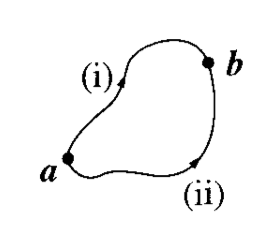
\includegraphics[width=0.95\textwidth]{./images/schematics/closed_path_integral_of_electric_field_is_0.png}
   \end{center}
  \end{column}
  \begin{column}{0.65\textwidth}
    \begin{equation*}
       \int_{a\;{\color{red}along\;i}}^{b} \vec{E} \cdot d\vec{\ell} = \int_{a\;{\color{red}along\;ii}}^{b} \vec{E} \cdot d\vec{\ell} \Rightarrow
    \end{equation*}
    \begin{equation*}
       \int_{a\;{\color{red}along\;i}}^{b} \vec{E} \cdot d\vec{\ell} = - \int_{b\;{\color{red}along\;ii}}^{a} \vec{E} \cdot d\vec{\ell} \Rightarrow
    \end{equation*}
    \begin{equation*}
       \oint \vec{E} \cdot d\vec{\ell} = 0
    \end{equation*}
  \end{column}
\end{columns}

\end{frame}


%
%
%

% starting reminder
{
\reminderslide


%
%
%

\begin{frame}{Reminder: Curl}

The curl ($\vec{\nabla} \times \vec{A}$) of a vector
field $\vec{A}$ = $\Big(A_x, A_y, A_z \Big)$ is defined as:
\begin{equation*}
     \vec{\nabla} \times \vec{A} =
       \left|
          \begin{array}{ccc}
             \hat{x} & \hat{y} & \hat{z} \\
             \frac{\partial}{\partial x}  & \frac{\partial}{\partial y} & \frac{\partial}{\partial z} \\
             A_x     & A_y     & A_z     \\
          \end{array}
       \right| =
       \Big( \frac{\partial A_z}{\partial y} - \frac{\partial A_y}{\partial z} \Big) \hat{x} -
       \Big( \frac{\partial A_z}{\partial x} - \frac{\partial A_x}{\partial z} \Big) \hat{y} +
       \Big( \frac{\partial A_y}{\partial x} - \frac{\partial A_x}{\partial y} \Big) \hat{z}
\end{equation*}

\begin{columns}
  \begin{column}{0.55\textwidth}
   \begin{center}
     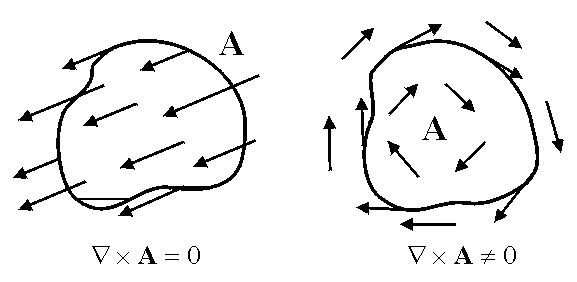
\includegraphics[width=0.95\textwidth]{./images/schematics/curl_1.png}
   \end{center}
  \end{column}
  \begin{column}{0.45\textwidth}
    The curl of a vector field, evaluated at a specific space point,
    tells us how much the field curls about that point.\\
  \end{column}
\end{columns}

\end{frame}

%
%
%

\begin{frame}{Reminder: Stokes' theorem}

Stokes' theorem {\bf relates
the circulation of a vector field $\vec{F}$ around a closed line C
with the flux of the curl of the vector field $\vec{F}$ through the open surface S} defined by the closed line C.\\

\vspace{0.5cm}

\begin{columns}
  \begin{column}{0.45\textwidth}
   \begin{center}
     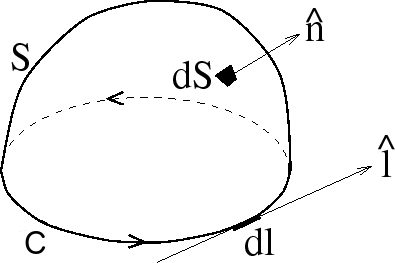
\includegraphics[width=0.95\textwidth]{./images/schematics/stokes_theorem_C.png}
   \end{center}
  \end{column}
  \begin{column}{0.45\textwidth}
  {\Large
    \begin{equation*}
      \oint_{C} \vec{F} \cdot d\vec{\ell} = \int_{S} (\vec{\nabla} \times \vec{F}) \cdot d\vec{S}
    \end{equation*}
  }
  \end{column}
\end{columns}

\end{frame}

} % end reminder

%
%
%

\begin{frame}{Circuital law for Electrostatics}

Applying the Stoke's theorem for the electric field $\vec{E}$ we have
\begin{equation*}
    \oint \vec{E} \cdot d\vec{\ell} = \int_{S} (\vec{\nabla} \times \vec{E}) \cdot d\vec{S}
\end{equation*}

But we know that for any closed path
\begin{equation*}
    \oint \vec{E} \cdot d\vec{\ell} = 0
\end{equation*}

Therefore
\begin{equation*}
    \int_{S} (\vec{\nabla} \times \vec{E}) \cdot d\vec{S} = 0
\end{equation*}

If the above is true for any surface S, then
\begin{equation*}
    \vec{\nabla} \times \vec{E} = 0
\end{equation*}

$\vec{E}$ is a {\em special} vector field: One that has {\bf no rotation} for all points in space.

\end{frame}


%
%
%

\begin{frame}{Our first two Maxwell equations for Electrostatics}

\begin{center}
 {\Large
  \begin{table}[H]
    \begin{tabular}{|l|c|c|}
      \hline
          & {\it Integral form} & {\it Differential form} \\
      \hline
      {\bf Gauss's law} &
        $\oint \vec{E} \cdot d\vec{S} = Q_{enclosed} / \epsilon_0$ &
        $\vec{\nabla} \cdot \vec{E} = \rho / \epsilon_0$ \\

      {\bf Circuital law} &
        $\oint \vec{E} \cdot d\vec{\ell} = 0$ &
        $\vec{\nabla} \times \vec{E} = 0$ \\
      \hline
    \end{tabular}
  \end{table}
 }
\end{center}

\end{frame}


%
%
%

\begin{frame}{Electric potential}

Now I will introduce the new concept of the {\bf electric potential (V)}.\\

\vspace{0.2cm}

\begin{itemize}
 \item {\bf Not be confused with electric potential energy (U)}. \\
       The choice of names is unfortunate.
\end{itemize}

\vspace{0.1cm}

We define the electric potential V at a position $\vec{r}$ to be the
{\bf amount of work required to bring a charge Q at position $\vec{r}$, divided by the charge Q}
\begin{equation*}
    V = \frac{W}{Q}
\end{equation*}

\vspace{0.1cm}

In SI, the potential has units of {\bf Volts} (V). \\
It is a derived unit: A Volt is a Joule per Coulomb (J/C).\\


\end{frame}

%
%
%

\begin{frame}{Electric potential}

The potential V is {\bf scalar field}:
\begin{itemize}
 \item
   Like $\vec{E}$, it permeates all space.
 \item
   Unlike $\vec{E}$, it associates a scalar (not a vector) with every space point.
\end{itemize}

\vspace{0.3cm}

The {\bf electric field $\vec{E}$ and the potential V are related} as follows:
\begin{equation*}
   \vec{E} = - \vec{\nabla} V
\end{equation*}

The fact that we can express $\vec{E}$, a vector field, as the gradient fo a scalar
field is due to a {\em special property} of $\vec{E}$.
We shall see that special property expressed in the {\em circuital law} in just a while.\\

\end{frame}

%
%
%

\begin{frame}{Electric potential of a point charge}

Assume that charge $q$ is at the origin and charge
$Q$ is brought at position $\vec{r}$.
As we saw earlier, the work $W$ done to bring $Q$ at $\vec{r}$ is:
\begin{equation*}
   W = \frac{q Q}{4\pi\epsilon_0 |\vec{r}|}
\end{equation*}

Therefore, the potential at position $\vec{r}$ due to charge $q$ is:
\begin{equation*}
   V = \frac{W}{Q} = \frac{q}{4\pi\epsilon_0 |\vec{r}|}
\end{equation*}

We can generalise the above, relaxing the requirement that the point charge
$q$ is at the origin. If, instead, $q$ is placed at position $\vec{r}^{\;\prime}$,
then the electric potential at $\vec{r}$ can be written as:
\begin{equation*}
   V = \frac{q}{4\pi\epsilon_0 |\vec{r}-\vec{r}^{\;\prime}|}
\end{equation*}

\end{frame}

%
%
%

\begin{frame}{Potential of group of charges / continuous distribution}

The potential at position $\vec{r}$
due to a point charge $q$ placed at $\vec{r}^{\;\prime}$ is:
\begin{equation*}
   V = \frac{q}{4\pi\epsilon_0 |\vec{r}-\vec{r}^{\;\prime}|}
\end{equation*}

\vspace{0.2cm}

Note that the {\bf potential obeys the superposition principle}.\\
\vspace{0.2cm}

Therefore, the potential at position $\vec{r}$
due to charges $q_1$, $q_2$,..., $q_N$ placed at
positions $\vec{r}_1$, $\vec{r}_2$,..., $\vec{r}_N$ is given by:
\begin{equation*}
   V = \frac{1}{4\pi\epsilon_0}
   \sum_{i=1}^{N} \frac{q_i}{|\vec{r}-\vec{r}_{i}|}
\end{equation*}

Similarly, the potential at position $\vec{r}$
due to a continuous charge distribution $\rho$ is given by:
\begin{equation*}
   V = \frac{1}{4\pi\epsilon_0}
     \int_{\tau^\prime} \frac{\rho(\vec{r}^{\;\prime})d\tau^\prime}{|\vec{r}-\vec{r}^{\;\prime}|}
\end{equation*}

\end{frame}


%-------------------------------------------------------------------------------
%
% Worked example
%

{
\problemslide

%
%
%

\begin{frame}{Worked example: Electric potential of circular arc of charge}

\begin{blockexmplque}{Question}
A plastic rod having a uniformly distributed charge $Q$ has been bent
into a circular arc of radius $R$ and central angle $\phi$.
With $V$=0 at infinity, what is the electric potential at $P$, the centre of
curvature of the rod?
\end{blockexmplque}

\vspace{0.2cm}

\begin{columns}
  \begin{column}{0.25\textwidth}
   \begin{center}
     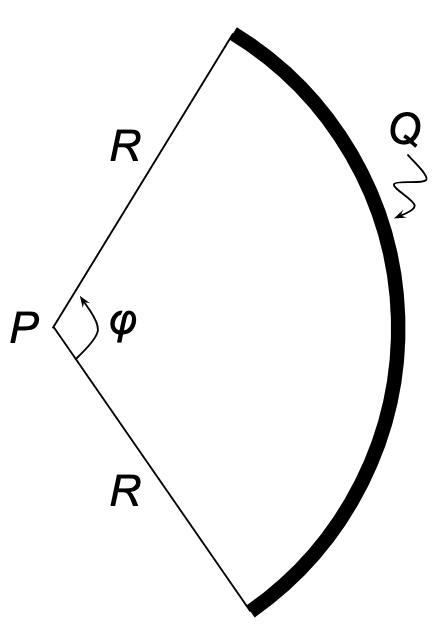
\includegraphics[width=0.99\textwidth]{./images/problems/lect03_potential_arc}
   \end{center}
  \end{column}
  \begin{column}{0.70\textwidth}
    Placing, for convenience but without loss of generality, the origin of the
    coordinate system at $P$, the potential at $\vec{r}=\vec{0}$ can be written as:
    \begin{equation*}
       V = \frac{1}{4\pi\epsilon_0}
         \int_{rod} \frac{dq(\vec{r}^{\;\prime})}{|\vec{r}^{\;\prime}|}
    \end{equation*}
    But $|\vec{r}^{\;\prime}|=R$ is a constant. Therefore:
    \begin{equation*}
       V = \frac{1}{4\pi\epsilon_0 R}
         \int_{rod} dq(\vec{r}^{\;\prime}) =
         \frac{Q}{4\pi\epsilon_0 R}
    \end{equation*}
  \end{column}
\end{columns}

\end{frame}

} % worked example

%-------------------------------------------------------------------------------
%
% Worked example
%

{
\problemslide

%
%
%

\begin{frame}{Worked example: Electric potential of non-conducting rod}

\begin{blockexmplque}{Question}
Thin non-conducting rod of length $L$ has a positive charge of uniform linear
density $\lambda$. Determine the electric potential $V$ due to the rod at point
$P$, at perpendicular distance $d$ from the left end of the rod.
\end{blockexmplque}

\begin{center}
  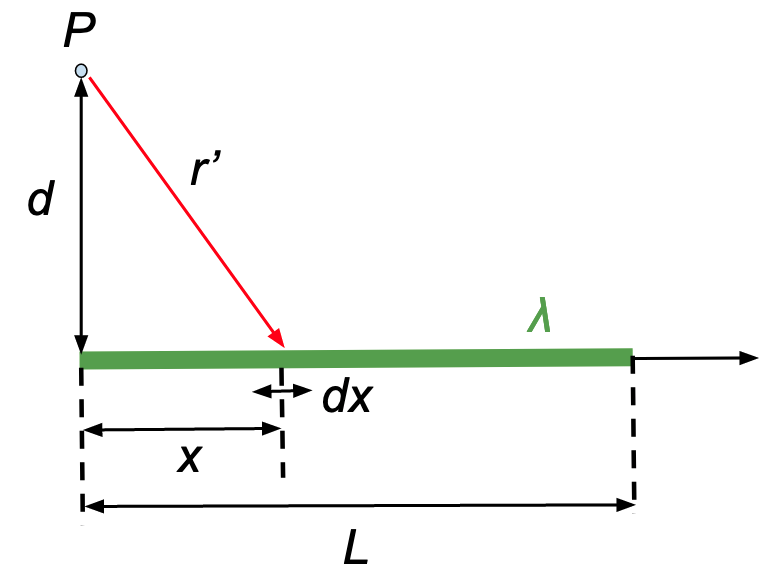
\includegraphics[width=0.60\textwidth]{./images/problems/lect03_potential_rod}
\end{center}

\end{frame}

%
%
%

\begin{frame}{Worked example: Electric potential of non-conducting rod}

Placing, for convenience but without loss of generality, the origin of the
coordinate system at $P$, the potential at $\vec{r}=\vec{0}$ can be written as:

\begin{equation*}
    V = \frac{1}{4\pi\epsilon_0} \int_{rod} \frac{dq(\vec{r}^{\;\prime})}{r^\prime}
\end{equation*}

\vspace{0.2cm}

The amount of charge $dq$ at position $\vec{r}^{\;\prime}$ is given by
$dq = \lambda dx$, therefore the potential becomes:
\begin{equation*}
    V = \frac{\lambda}{4\pi\epsilon_0} \int_{0}^{L} \frac{dx}{r^\prime}
\end{equation*}

To carry out the integration, we need to relate $r^\prime$ and $x$.
From the previous schematic, we find:
\begin{equation*}
    x^2 + d^2 = r^2 \Rightarrow r = \sqrt{x^2 + d^2}
\end{equation*}

\end{frame}

%
%
%

\begin{frame}{Worked example: Electric potential of non-conducting rod}

Therefore the potential can be written as:

\begin{equation*}
    V = \frac{\lambda}{4\pi\epsilon_0} \int_{0}^{L} \frac{dx}{\sqrt{x^2 + d^2}} =
        \frac{\lambda}{4\pi\epsilon_0} ln\Big(x + \sqrt{x^2+d^2}\Big)\Bigg\rvert_{0}^{L}
\end{equation*}

Evaluating the integral, we have:
\begin{equation*}
    V = \frac{\lambda}{4\pi\epsilon_0} ln\Big(x + \sqrt{x^2+d^2}\Big)\Bigg\rvert_{0}^{L} \Rightarrow
\end{equation*}
\begin{equation*}
    V = \frac{\lambda}{4\pi\epsilon_0} \Bigg\{ ln\Big(L + \sqrt{L^2+d^2}\Big) - ln\Big(d\Big) \Bigg\} \Rightarrow
\end{equation*}
\begin{equation*}
    V = \frac{\lambda}{4\pi\epsilon_0} ln\Big(\frac{L + \sqrt{L^2+d^2}}{d}\Big)
\end{equation*}


\end{frame}


} % worked example

%-------------------------------------------------------------------------------


%
%
%

\begin{frame}{A p.d.e. (*) for the electric potential}

Let's consider what is involved in calculating $\vec{E}$:
Since it is a vector field we need to calculate all three components
($E_x$,$E_y$ and $E_z$).\\

\vspace{0.2cm}
We have already seen that (Gauss's law; 1$^{st}$ Maxwell equation):
\begin{equation*}
  \vec{\nabla} \cdot \vec{E} = \frac{\rho}{\epsilon_0}
\end{equation*}

On its own, the divergence of a vector field is
{\bf not enough to uniquely determine} that vector field.\\
However, in this lecture, we also saw another differential equation for
$\vec{E}$ (Circuital law; 2$^{nd}$ Maxwell equation):
\begin{equation*}
  \vec{\nabla} \times \vec{E} = 0
\end{equation*}

So we have {\bf two coupled differential equations to compute $\vec{E}$}:\\
The components of $\vec{E}$ are {\bf interdependent}.
It all sounds too complicated!

\vspace{0.2cm}

\noindent\rule{2cm}{0.4pt}\\
{\scriptsize
 (*) {\it p.d.e.: partial differential equation.}
}

\end{frame}

%
%
%

\begin{frame}{A p.d.e. for the electric potential}

Can we simplify things?

\begin{itemize}
  \item Let's start by exploiting the fact that:
        \begin{equation*}
           \vec{\nabla} \times \vec{E} = 0
        \end{equation*}
  \item We know (see your basic calculus textbooks)
        that {\bf the curl of the gradient of any scalar function $\lambda$ is always 0}:
        \begin{equation*}
           \vec{\nabla} \times \Big( \vec{\nabla} \lambda \Big) = 0
        \end{equation*}
  \item So, $\vec{E}$ is the gradient of a scalar function $\lambda$ ($\vec{E} = \vec{\nabla} \lambda$).
  \item We already know which is that scalar function.
        It is the electric potential V introduced earlier ($\lambda = -V$):
        \begin{equation*}
           \vec{E} = - \vec{\nabla} V
        \end{equation*}
        The minus sign is conventional.
\end{itemize}

\end{frame}

%
%
%

\begin{frame}{A p.d.e. for the electric potential: The Poisson equation}

So we can {\bf reduce the problem of calculating $\vec{E}$}
(a vector for which we need to calculate all 3 components $E_x$, $E_y$ and $E_z$)
{\bf to the simpler problem of calculating a single scalar function V}.\\
\vspace{0.3cm}

Starting from Gauss's law, and substituting $\vec{E} = - \vec{\nabla} V$ we have:
\begin{equation*}
  \vec{\nabla} \cdot \vec{E} = \frac{\rho}{\epsilon_0} \Rightarrow
  \vec{\nabla} \cdot \Big( - \vec{\nabla} V \Big) = \frac{\rho}{\epsilon_0} \Rightarrow
\end{equation*}
\begin{equation*}
  \vec{\nabla}^{2} V = - \frac{\rho}{\epsilon_0}
\end{equation*}

The above is known as the {\bf Poisson equation}.\\
\vspace{0.3cm}

($\vec{\nabla}^{2} = \frac{\partial^2}{\partial x^2} + \frac{\partial^2}{\partial y^2} + \frac{\partial^2}{\partial z^2}$
is known as the {\em Laplace operator} - see later).

\end{frame}

%
%
%

\begin{frame}{A p.d.e. for the electric potential: The Laplace equation}

We are often interested in {\bf finding the electric field away from charges}
(in regions where the charge density $\rho$ is 0).\\
\vspace{0.3cm}
Then, Poisson's equation:
\begin{equation*}
  \vec{\nabla}^{2} V = - \frac{\rho}{\epsilon_0}
\end{equation*}

becomes:
\begin{equation*}
  \vec{\nabla}^{2} V = 0
\end{equation*}

\vspace{0.3cm}
The above is known as the {\bf Laplace equation}.

\end{frame}

%
%
%

% starting reminder
{
\reminderslide

%
%
%

\begin{frame}{Reminder: The Laplace operator}

The Laplace operator is a 2$^{nd}$ order differential operator defined as follows:
\begin{equation*}
  \vec{\nabla}^{2} = \frac{\partial^2}{\partial x^2} + \frac{\partial^2}{\partial y^2} + \frac{\partial^2}{\partial z^2}
\end{equation*}

So the Laplacian of a scalar function f is:
\begin{equation*}
  \vec{\nabla}^{2}f = \frac{\partial^2 f}{\partial x^2} + \frac{\partial^2 f}{\partial y^2} + \frac{\partial^2 f}{\partial z^2}
\end{equation*}

The Laplacian {\bf is the divergence of the gradient} of the scalar function f:
\begin{equation*}
  \vec{\nabla}^{2} f =  \vec{\nabla} \cdot \Big( \vec{\nabla} f \Big)
\end{equation*}

It represents a quantity which is important in several physical processes:\\
The Laplacian $\vec{\nabla}^{2} f(\vec{r})$ of a scalar function f at a point $\vec{r}$
tells you {\bf how much $f(\vec{r})$ differs from its average over a small volume around $\vec{r}$.}

\end{frame}

} % end reminder


%
% Worked example
%

{
\problemslide

%
%
%

\begin{frame}{Worked example: Finding $\rho$ from V}

\begin{blockexmplque}{Question}
  A potential V is given by:
  \begin{equation*}
     V(\vec{r}) = V(r) = V_{0} e^{-(r/a)^2}
  \end{equation*}
  where $r = |\vec{r}| = \sqrt{x^2+y^2+z^2}$.\\
  Find out the charge density $\rho$ that is responsible for it.
\end{blockexmplque}

\vspace{0.1cm}

Starting from  Poisson's equation we can solve for $\rho$:
\begin{equation*}
  \vec{\nabla}^{2}V(\vec{r}) = -\rho(\vec{r})/\epsilon_0 \Rightarrow
  \rho(\vec{r}) = - \epsilon_0 \vec{\nabla}^{2}V(\vec{r})
\end{equation*}

\vspace{0.1cm}

The Laplacian of V is:
\begin{equation*}
   \vec{\nabla}^{2}V =
     \Big( \frac{\partial^2}{\partial x^2} +
           \frac{\partial^2}{\partial y^2} +
           \frac{\partial^2}{\partial z^2}
     \Big) V =
     V_0
     \Big(
      \frac{\partial^2 e^{-(r/a)^2}}{\partial x^2} +
      \frac{\partial^2 e^{-(r/a)^2}}{\partial y^2} +
      \frac{\partial^2 e^{-(r/a)^2}}{\partial z^2}
     \Big)
\end{equation*}

\end{frame}

%
%
%

\begin{frame}{Worked example: Finding $\rho$ from V}

Using the chain rule
\begin{equation*}
   \frac{\partial e^{-(r/a)^2}}{\partial x} =
          \frac{\partial r}{\partial x} \frac{\partial}{\partial r} e^{-(r/a)^2}
\end{equation*}

where
\begin{equation*}
   \frac{\partial r}{\partial x} = \frac{\partial}{\partial x} (x^2+y^2+z^2)^{1/2} =
      \frac{1}{2} (x^2+y^2+z^2)^{-1/2} 2x = \frac{x}{r}
\end{equation*}

and
\begin{equation*}
   \frac{\partial}{\partial r} e^{-(r/a)^2} =
       e^{-(r/a)^2} \frac{\partial}{\partial r} \Big( -\frac{r^2}{a^2} \Big) =
       e^{-(r/a)^2} \Big( \frac{-2r}{a^2} \Big)
\end{equation*}

Therefore
\begin{equation*}
   \frac{\partial e^{-(r/a)^2}}{\partial x} = -\frac{2x}{a^2} e^{-(r/a)^2}
\end{equation*}

\end{frame}


%
%
%

\begin{frame}{Worked example: Finding $\rho$ from V}

Continuing, in the same manner, to compute the
The second partial derivative wrt to x of $e^{-(r/a)^2}$ is:
\begin{equation*}
   \frac{\partial^2}{\partial x^2} e^{-(r/a)^2} =
   \frac{\partial}{\partial x} \Big( \frac{\partial}{\partial x} e^{-(r/a)^2} \Big)
\end{equation*}

We already calculated (see previous page) that:
\begin{equation*}
   \frac{\partial}{\partial x} e^{-(r/a)^2} = -\frac{2x}{a^2} e^{-(r/a)^2}
\end{equation*}

Therefore:
\begin{equation*}
   \frac{\partial^2}{\partial x^2} e^{-(r/a)^2} =
   \frac{\partial}{\partial x} \Big( -\frac{2x}{a^2} e^{-(r/a)^2} \Big) =
   \Big(- \frac{2}{a^2} \frac{\partial}{\partial x} x \Big) e^{-(r/a)^2}
   - \frac{2x}{a^2} \Big(\frac{\partial}{\partial x} e^{-(r/a)^2} \Big)
\end{equation*}
\begin{equation*}
   = -\frac{2}{a^2} e^{-(r/a)^2} - \frac{2x}{a^2} \Big( -\frac{2x}{a^2} e^{-(r/a)^2} \Big) = \Big( \frac{4x^2}{a^4} - \frac{2}{a^2} \Big) e^{-(r/a)^2}
\end{equation*}

\end{frame}


%
%
%

\begin{frame}{Worked example: Finding $\rho$ from V}

Similarly:
\begin{equation*}
   \frac{\partial^2}{\partial y^2} e^{-(r/a)^2} =
     \Big( \frac{4y^2}{a^4} - \frac{2}{a^2} \Big) e^{-(r/a)^2} \;\;and\;\;
   \frac{\partial^2}{\partial z^2} e^{-(r/a)^2} =
     \Big( \frac{4z^2}{a^4} - \frac{2}{a^2} \Big) e^{-(r/a)^2}
\end{equation*}

\vspace{0.1cm}

Therefore:
\begin{equation*}
  \vec{\nabla}^{2} V
     = V_{0} \vec{\nabla}^{2} e^{-(r/a)^2}
     = V_{0} \Big( 4\frac{x^2+y^2+z^2}{a^4} - \frac{6}{a^2} \Big)  e^{-(r/a)^2} \Rightarrow
\end{equation*}
\begin{equation*}
  \vec{\nabla}^{2} V
     = V_{0} \Big( \frac{4r^2}{a^4} - \frac{6}{a^2} \Big)  e^{-(r/a)^2}
\end{equation*}

\vspace{0.1cm}

So, finally, the charge density is given by:
\begin{equation*}
  \rho(r) = -\epsilon_0 \vec{\nabla}^{2} V(r) = -\epsilon_0 V_{0} \Big( \frac{4r^2}{a^4} - \frac{6}{a^2} \Big)  e^{-(r/a)^2}
\end{equation*}

\noindent\rule{2cm}{0.4pt}\\
{\scriptsize
Since the problem has spherical symmetry ($V(\vec{r})$ is a function of $r=|\vec{r}|$ alone)
it would have been easier to use the Laplacian operator in spherical coordinates (Try this on your own):
$\vec{\nabla}^{2} =
    \frac{1}{r^2} \frac{\partial}{\partial r} \Big( r^2 \frac{\partial}{\partial r} \Big) +
    \frac{1}{r^2 sin^{2}\phi} \frac{\partial^{2}}{\partial {\theta}^{2}} +
    \frac{1}{r^2 sin\phi} \frac{\partial}{\partial \phi} \Big( sin\phi \frac{\partial}{\partial \phi} \Big)$.
}

\end{frame}

} % Examples

%
%
%

\begin{frame}{Solving Poisson's equation}

Previously, we used Poisson's equation to solve a simple problem:
We found the charge density $\rho(\vec{r})$ responsible for a particular potential V($\vec{r}$).\\

\vspace{0.2cm}

In practical applications we are usually interested in the {\em inverse} problem:
We start from a known charge density and want to calculate the potential.\\

\vspace{0.2cm}

Unfortunately, the Poisson equation is {\em the wrong way around}.
\begin{equation*}
   \vec{\nabla}^{2} V(\vec{r}) = -\frac{\rho(\vec{r})}{\epsilon_0}
\end{equation*}

Whereas one simply needs to differentiate the potential to get the density,
one needs to invert the Poisson equation to compute the potential:

\begin{equation*}
   V(\vec{r}) = \frac{1}{4\pi\epsilon_0} \int \frac{\rho(\vec{r^{\prime}})}{|\vec{r}-\vec{r^{\prime}}|} d^{3}r^{\prime}
\end{equation*}

\end{frame}


%
%
%

\begin{frame}{Solving Poisson's equation}

{\em Inverting} the Poisson equation gives us:
\begin{equation*}
   V(\vec{r}) = \frac{1}{4\pi\epsilon_0} \int \frac{\rho(\vec{r^{\prime}})}{|\vec{r}-\vec{r^{\prime}}|} d^{3}r^{\prime}
\end{equation*}

In general, it is not easy to calculate this integral analytically.\\
\begin{itemize}
  \item
   Moreover, in some practical applications, we may not know the density $\rho$ \underline{everywhere} in space.
   We may know only V at some boundaries of the region of interest.\\
\end{itemize}
\vspace{0.2cm}

It is usually preferable to look at a problem in its differential form:\\
\vspace{0.2cm}

{\bf
The Poisson equation
$\vec{\nabla}^{2} V(\vec{r}) = -\frac{\rho(\vec{r})}{\epsilon_0}$
together with appropriate boundary conditions is equivalent to the above integral}.\\

\vspace{0.2cm}

Notice that without the appropriate boundary conditions,
the Poisson equation by itself does not determine V.

\end{frame}


%
%
%

\begin{frame}{Boundary conditions}

Take the Poisson equation in the absence of charges (Laplace equation).\\
For now, let's just consider the 1-dimensional case:
\begin{equation*}
  \frac{d^{2}V(x)}{dx^2} = 0
\end{equation*}
One can easily solve the above and obtain:
\begin{equation*}
  \frac{d^{2}V(x)}{dx^2} = 0 \Rightarrow \frac{dV(x)}{dx} = c_{1} \Rightarrow V(x) = c_{1}x + c_{2}
\end{equation*}

The above is not a solution, but a {\bf class of solutions}.\\
\vspace{0.2cm}

The exact solution is known if I can determine the constants $c_1$ and $c_2$.\\
For example, I can determine $c_1$, $c_2$ if I know:
\begin{itemize}
  \item the value of V(x) at 2 points, or
  \item or, the derivative and the value of V(x) at 1 point.
\end{itemize}

\end{frame}


%
%
%

\begin{frame}{Boundary conditions}

How about the Laplace equation at higher dimensions?\\
\vspace{0.2cm}

As we have seen, in the usual 3 dimensions we have:
\begin{equation*}
  \vec{\nabla}^{2} V(\vec{r}) =
    \frac{\partial^{2}V(x,y,z)}{\partial x^2} +
    \frac{\partial^{2}V(x,y,z)}{\partial y^2} +
    \frac{\partial^{2}V(x,y,z)}{\partial z^2} = 0
\end{equation*}

The main question is:
{\bf What are the appropriate boundary conditions now that there are partial derivatives involved?}\\
\vspace{0.2cm}

This is a much harder problem:
\begin{itemize}
  \item Not a finite number of constants in the solution!
  \item Not easy to say whether a set of boundary conditions is acceptable.
\end{itemize}

\end{frame}


%
%
%

\begin{frame}{Uniqueness theorem}

{\bf
 A uniqueness theorem is a proof that a given set of boundary conditions is sufficient.
}
\begin{itemize}
{\small
  \item It guarantees that a set of boundary conditions yields a unique solution.
}
\end{itemize}

\vspace{0.2cm}

The simpler set of boundary conditions
is the so-called {\bf Dirichlet} boundary condition:
The value of V is specified everywhere on the (closed) boundary surface S
of the volume where we are interested to know V.
\begin{itemize}
{\small
  \item The statement that the above boundary conditions yield a unique solution
         is usually referred to as the {\bf first uniquness theorem}.
}
\end{itemize}

\vspace{0.4cm}

\noindent\rule{2cm}{0.4pt}\\
{\small
Notice a ramification of the uniquness theorem:
It doesn't matter how arrive at a solution (by mathematical genius or luck).
If you have a solution that satisfies the given boundary conditions
then that is {\em the only} solution.\\
}

\end{frame}


%
% What to remember
%

\renewcommand{\lecturesummarytitle}{Main points to remember }

\renewcommand{\summarizedlecture}{3 }

%
%
%

\begin{frame}{Lecture \summarizedlecture - \lecturesummarytitle}

\begin{itemize}
\item {\bf To bring together a collection of charges I need to do work}
      (for example, In case of two like-sign charges I need to exert a force against the action of the field)
      \begin{equation*}
        W = \int \vec{F} \cdot d\vec{\ell}
      \end{equation*}
\item The work done can be positive or negative.
\item The work done is {\bf path-independent}
  \begin{itemize}
     \item I do the same work regardless of the path followed to bring the charges in their positions.
     \item We say that the electric force is {\bf conservative}.
  \end{itemize}
\item The work done is converted to {\bf electric potential energy}
\item We calculated the  potential energy for systems of 2, 3 and N charges as well as continuous distributions of charge.

\end{itemize}

\end{frame}

%
%
%

\begin{frame}{Lecture \summarizedlecture - \lecturesummarytitle (cont'd)}

For a
\begin{itemize}
\item system of 2 charges:
 \begin{equation*}
      U = \frac{q_1 q_2}{4\pi\epsilon_0} \frac{1}{|\vec{r}_{12}|}
 \end{equation*}

\item system of 3 charges:
 \begin{equation*}
   U = \frac{q_1 q_2}{4\pi\epsilon_0} \frac{1}{|\vec{r}_{12}|} +
       \frac{q_1 q_3}{4\pi\epsilon_0} \frac{1}{|\vec{r}_{13}|} +
       \frac{q_2 q_3}{4\pi\epsilon_0} \frac{1}{|\vec{r}_{23}|}
 \end{equation*}

\item system of N charges:
 \begin{equation*}
   U = \frac{1}{2} \sum_{i,j=1;i{\ne}j}^{N} \frac{q_i q_j}{4\pi\epsilon_0|\vec{r}_{ij}|}
 \end{equation*}

\item continuous charge distribution (with density $\rho$ over a volume $\tau$):
 \begin{equation*}
    U = \frac{1}{2} \int_{\tau} d\tau \int_{\tau^{\prime}} d\tau^{\prime}
        \frac{\rho(\vec{r}) \rho(\vec{r^{\prime}})}{4\pi\epsilon_0|\vec{r} - \vec{r^{\prime}}|}
 \end{equation*}

\end{itemize}

\end{frame}

%
%
%

\begin{frame}{Lecture \summarizedlecture - \lecturesummarytitle (cont'd)}

\begin{itemize}
  \item
  The electric {\bf potential energy is stored in the electric field}:
  \begin{equation*}
     U = \frac{\epsilon_0}{2} \int_{all\;space} |\vec{E}(\vec{r})|^2  d\tau
  \end{equation*}

  \item
  {\bf Relationship between force and potential energy}:\\
  \begin{equation*}
     U = \int \vec{F} \cdot d\vec{\ell}
  \end{equation*}
  \begin{equation*}
     \vec{F} = -\vec{\nabla}U
  \end{equation*}

  \item
  {\bf Electric potential (V)}: A scalar field
      \begin{itemize}
          \item It is the amount of work required to bring a charge Q at position $\vec{r}$, divided by the charge Q.
          \item SI units: Volts (V)
            \begin{itemize}
               \item Derived unit: One Joule per Coulomb
            \end{itemize}
      \end{itemize}
\end{itemize}

\end{frame}

%
%
%

\begin{frame}{Lecture \summarizedlecture - \lecturesummarytitle (cont'd)}

\begin{itemize}
  \item We also studied the {\bf circuital law for Electrostatics}
     \begin{itemize}
        \item Our second set of Maxwell's equations.
     \end{itemize}
  \vspace{0.2cm}
  \item Maxwell's equation we know so far:
\end{itemize}

\begin{center}
 {
  \begin{table}[H]
    \begin{tabular}{|l|c|c|}
      \hline
          & {\it Integral form} & {\it Differential form} \\
      \hline
      {\bf Gauss's law} &
        $\oint \vec{E} \cdot d\vec{S} = Q_{enclosed} / \epsilon_0$ &
        $\vec{\nabla} \cdot \vec{E} = \rho / \epsilon_0$ \\

      {\bf Circuital law} &
        $\oint \vec{E} \cdot d\vec{\ell} = 0$ &
        $\vec{\nabla} \times \vec{E} = 0$ \\
      \hline
    \end{tabular}
  \end{table}
 }
\end{center}

\begin{itemize}
  \item Because (in Electrostatics) the electric field has no rotation
        it can be expressed as the gradient of a scalar function (the electric potential):
        \begin{equation*}
           \vec{E} = - \vec{\nabla} V
        \end{equation*}
\end{itemize}


\end{frame}

%
%
%

\begin{frame}{Lecture \summarizedlecture - \lecturesummarytitle (cont'd)}

\begin{itemize}

  \item Need both the divergence and the curl of $\vec{E}$ (both Gauss' and circuital laws)
        to determine all three components of $\vec{E}$.
    \begin{itemize}
    {
      \item Gauss' and circuital laws provide a coupled system of 1$^{st}$ order p.d.e's.
    }
    \end{itemize}

  \item I can combine the Gauss' and circuital laws into a single 2$^{nd}$ order p.d.e for the
        electric potential V: {\bf Poisson equation}
        \begin{equation*}
           \vec{\nabla}^{2} V = - \frac{\rho}{\epsilon_0}
        \end{equation*}

  \item Away from sources ($\rho$=0) Poisson's equation becomes $\vec{\nabla}^{2} V = 0$
        which is known as the {\bf Laplace equation}.

  \item Using the Poisson (or Laplace) equations one can determine V (and, thus, $\vec{E}$)
        only using the appropriate {\bf boundary conditions}.

  \item {\bf A uniqueness theorem} is a proof that a given set of boundary conditions is sufficient.

\end{itemize}

\end{frame}


%
% At the next lecture
%

\begin{frame}{At the next lecture (Lecture \nextlecture)}

{\bf What happens when materials are placed in an electric field}?\\

\vspace{0.2cm}

We will study the two main types of materials with regards to their electrical properties:
\begin{itemize}
  \item Conductors
  \item Dielectrics (or insulators)
\end{itemize}

\vspace{0.2cm}
and we will discuss some useful concepts:

\begin{itemize}
  \item Capacitance
  \item The electric dipole
  \item Polarization
\end{itemize}

\end{frame}

%
% Optional reading
%

%
% Optional reading
%

\begin{frame}[plain,c]
\begin{center}
{\Huge \bf Optional reading for Lecture \thislecture}
\end{center}
\end{frame}


%
%
%

\begin{frame}{The electrostatic potential energy is stored in the field}

We can now prove a statement I made earlier: That {\bf the electrostatic potential energy is stored in the electric field}.\\
\vspace{0.1cm}
The potential energy stored in a system of N charges can be written as:
\begin{equation*}
   U = \frac{1}{2} \sum_{i,j=1;i{\ne}j}^{N} \frac{q_i q_j}{4\pi\epsilon_0|\vec{r}_{ij}|}
     = \frac{1}{2} \sum_{i}^{N} q_i {\color{red}\sum_{j=1;j{\ne}i}^{N} \frac{q_j}{4\pi\epsilon_0|\vec{r}_{ij}|}}
     = \frac{1}{2} \sum_{i}^{N} q_i {\color{red}V(\vec{r}_{i})}
\end{equation*}

where
\begin{equation*}
   V(\vec{r}_{i}) = \sum_{j=1;j{\ne}i}^{N} \frac{q_j}{4\pi\epsilon_0|\vec{r}_{ij}|}
\end{equation*}
is the potential at $\vec{r}_{i}$ due to all charges other than $q_i$.\\

\vspace{0.2cm}

The above result can be adapted for the continuous case too, using the (by now) familiar substitutions:
\begin{equation*}
   U = \frac{1}{2} \sum_{i}^{N} q_i V(\vec{r}_{i}) \rightarrow \frac{1}{2} \int_{V} \rho(\vec{r}) V(\vec{r}) d\tau
\end{equation*}

\end{frame}

%
%
%

\begin{frame}{The electrostatic potential energy is stored in the field}

The expression we have for the potential energy U of a continuous charge
distribution described by charge density $\rho$ is:
\begin{equation*}
   U = \frac{1}{2} \int_{V} \rho(\vec{r}) V(\vec{r}) d\tau
\end{equation*}
We will show that U is related to a volume integral of $|\vec{E}|^2$.\\

\vspace{0.3cm}

Using Gauss's law, the charge density $\rho$ can be written as:
\begin{equation*}
   \vec{\nabla} \vec{E}(\vec{r}) = \frac{\rho(\vec{r})}{\epsilon_0} \Rightarrow \rho(\vec{r}) = \epsilon_0 \vec{\nabla} \vec{E}(\vec{r})
\end{equation*}

Substituting $\rho$ into the expression for U, we have:
\begin{equation*}
   U = \frac{\epsilon_0}{2} \int_{V} \Big(\vec{\nabla} \vec{E}(\vec{r})\Big) V(\vec{r}) d\tau
\end{equation*}

\end{frame}

%
%
%

\begin{frame}{The electrostatic potential energy is stored in the field}

I would like to express U in terms of $\vec{E}$ only.\\
\vspace{0.2cm}
Since $\vec{\nabla} V = - \vec{E}$, I will try to move the $\vec{\nabla}$ in the previous
expression so that it operates on V instead on $\vec{E}$.\\
\vspace{0.2cm}
The trick is to operate with $\vec{\nabla}$ on the product $\vec{E} V$:
\begin{equation*}
  \vec{\nabla} \Big(\vec{E}(\vec{r}) V(\vec{r}) \Big) =
     \Big(\vec{\nabla} \vec{E}(\vec{r}) \Big) V(\vec{r}) + \vec{E}(\vec{r}) \Big(\vec{\nabla} V(\vec{r}) \Big) \Rightarrow
\end{equation*}
\begin{equation*}
   \Big(\vec{\nabla} \vec{E}(\vec{r}) \Big) V(\vec{r}) =
      \vec{\nabla} \Big(\vec{E}(\vec{r})) V(\vec{r}) \Big) - \vec{E}(\vec{r}) \Big(\vec{\nabla} V(\vec{r}) \Big)
\end{equation*}

Substituting the above in the last equation of the previous page we have:
\begin{equation*}
   U = \frac{\epsilon_0}{2} \int_{V} \vec{\nabla} \Big(\vec{E}(\vec{r})) V(\vec{r}) \Big) d\tau -
       \frac{\epsilon_0}{2} \int_{V} \vec{E}(\vec{r}) \Big(\vec{\nabla} V(\vec{r}) \Big)  d\tau
\end{equation*}

\end{frame}


%
%
%

\begin{frame}{The electrostatic potential energy is stored in the field}

Using Gauss' theorem, the 1$^{st}$ term of the previous expression for U becomes:
\begin{equation*}
   \int_{V} \vec{\nabla} \Big(\vec{E}(\vec{r})) V(\vec{r}) \Big) d\tau =
   \oint_{S} \Big(\vec{E}(\vec{r})) V(\vec{r}) \Big) d\vec{S}
\end{equation*}

Using $\vec{\nabla} V = - \vec{E}$, the 2$^{nd}$ term of the previous expression for U becomes:
\begin{equation*}
   \int_{V} \vec{E}(\vec{r}) \Big(\vec{\nabla} V(\vec{r}) \Big) d\tau =
  -\int_{V} \vec{E}(\vec{r}) \vec{E}(\vec{r}) d\tau =
  -\int_{V} |\vec{E}(\vec{r})|^{2} d\tau
\end{equation*}

The equation for the electric potential U can be rewritten as:
\begin{equation*}
   U = \frac{\epsilon_0}{2} \oint_{S} \Big(\vec{E}(\vec{r})) V(\vec{r}) \Big) d\vec{S} +
       \frac{\epsilon_0}{2} \int_{V} |\vec{E}(\vec{r})|^2  d\tau
\end{equation*}

As r $\rightarrow\infty$, the surface term $\oint_{S} \Big(...\Big) d\vec{S}$ $\rightarrow$ 0.
Therefore:
\begin{equation*}
   U = \frac{\epsilon_0}{2} \int_{all\;space} |\vec{E}(\vec{r})|^2  d\tau
\end{equation*}

\end{frame}


%
%
%

\begin{frame}{The Dirichlet boundary condition yields unique solutions}

This can be understood as follows:\\
\begin{itemize}
{\small
  \item Imagine a volume with a charge density $\rho$ which is known at all points.
  \item Also assume that the potential is known everywhere on the boundaries (i.e. on the surface surrounding the volume)
  \item Assume that there are two distinct solutions, $V_{1}(\vec{r})$ and $V_{2}(\vec{r})$.
    \begin{itemize}
    {\small
       \item $\vec{\nabla}^{2}V_1(\vec{r}) = -\rho(\vec{r})/\epsilon_0$
       \item $\vec{\nabla}^{2}V_2(\vec{r}) = -\rho(\vec{r})/\epsilon_0$
    }
    \end{itemize}
  \item Now, consider the function $V_{3}(\vec{r}) = V_{1}(\vec{r}) - V_{2}(\vec{r})$
    \begin{itemize}
    {\small
      \item At the boundary, $V_{3}(\vec{r}) = 0$ (since both $V_1$, $V_2$ satisfy the same boundary condition)
      \item Also, $V_{3}(\vec{r})$ satisfies the equation $\vec{\nabla}^{2}V_{3} = 0$ and, as such, changes monotonically inside the volume and has no minima/maxima.
    }
    \end{itemize}
  \item $V_3$ ranges between 0 and ...0, so $V_3$ is 0 everywhere in the given volume.
  \item This contradicts the assumption that two distinct solutions $V_1$, $V_2$ can exist.
        $V_1 = V_2$ everywhere in the volume, so a unique solution exists.
    \begin{equation*}
      \vec{\nabla}^{2}V_{3} = \vec{\nabla}^{2}(V_1-V_2) = \vec{\nabla}^{2}V_1 - \vec{\nabla}^{2}V_2 = - \frac{\rho}{\epsilon_0} + \frac{\rho}{\epsilon_0} = 0
    \end{equation*}
}
\end{itemize}

\end{frame}

%
%
%

{
\programmingslide

%
%
%

\begin{frame}{PHYS201 scientific programming task for Lecture \thislecture}

{\small

We will attempt to {\bf solve numerically the Laplace equation in 2-D},
for some given boundary conditions, and determine the potential V!\\
\vspace{0.2cm}
The Laplace equation in 2-D takes the form
\begin{equation*}
  \frac{\partial^2 V(x,y)}{\partial x^2} +
  \frac{\partial^2 V(x,y)}{\partial y^2} = 0
\end{equation*}
\vspace{0.2cm}
We will solve this equation for all x, y in the square area defined by:
\begin{equation*}
    0 < x < L \;\;\; \text{and} \;\;\; 0 < y < L
\end{equation*}
\vspace{0.2cm}
Our boundary conditions are:
\begin{equation*}
    V(x,0) = V_0, \;\;\; V(x,L) = 0,  \;\;\; V(0,y) = 0,  \;\;\; V(L,y) = 0
\end{equation*}
Take L = 1 m and V$_0$ = 1 V.
}
\end{frame}

%
%
%

\begin{frame}{PHYS201 scientific programming task for Lecture \thislecture}

{\small

{\bf \color{red}Hint:} Solve the Laplace equation numerically,
using the {\em finite difference method}.

Consider the Taylor expansions of a function f(x) around x:
\begin{equation*}
   f(x+h) = f(x) + h f^{\prime}(x) + \frac{h^2}{2} f^{\prime \prime}(x) + O(h^3)
\end{equation*}
\begin{equation*}
   f(x-h) = f(x) - h f^{\prime}(x) + \frac{h^2}{2} f^{\prime \prime}(x) - O(h^3)
\end{equation*}
where h is a small distance.\\
\vspace{0.2cm}
Adding the two equations, we obtain the
{\em first central difference approximation} for the second derivative of f(x):
\begin{equation*}
   f(x+h) + f(x-h) = 2f(x) + h^2 f^{\prime \prime}(x) + O(h^4) \Rightarrow
\end{equation*}
\begin{equation*}
   f^{\prime \prime}(x) = \frac{f(x+h) - 2f(x) + f(x-h)}{h^2} + O(h^2)
\end{equation*}
}
\end{frame}

%
%
%

\begin{frame}{PHYS201 scientific programming task for Lecture \thislecture}

{\small

\begin{columns}
  \begin{column}{0.25\textwidth}
   \begin{center}
     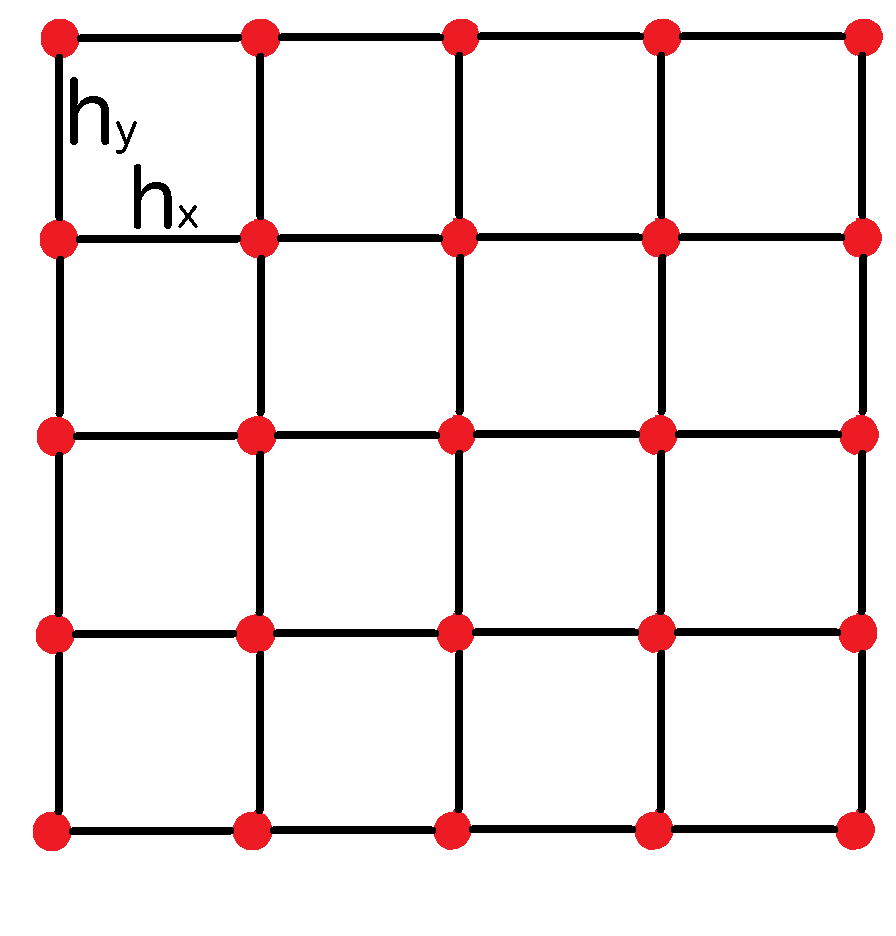
\includegraphics[width=0.90\textwidth]{./images/problems/lect03_computing_grid2d.png}
   \end{center}
  \end{column}
  \begin{column}{0.75\textwidth}
    Now, consider a uniform mesh (grid), as shown on the left,
    where the spacing between neighbouring points along x is h$_x$
    and the spacing between neighbouring points along y is h$_y$.\\
    \vspace{0.2cm}
    Using the {\em first central difference approximation},
    the Laplace equation for any point on the 2-D grid can be written as:
  \end{column}
\end{columns}

\begin{equation*}
   \frac{V(x+h_x,y) - 2V(x,y) + V(x-h_x, y)}{h_x^2} +
   \frac{V(x,y+h_y) - 2V(x,y) + V(x, y-h_y)}{h_y^2} = 0
\end{equation*}

If the grid is uniform (h$_x$ = h$_y$ = h), then the above equation becomes:
\begin{equation*}
   V(x+h,y) + V(x-h, y) +
   V(x,y+h) + V(x, y-h) - 4V(x,y) = 0
\end{equation*}

You have a set of such equations, one for each grid point, which you need
to {\bf solve simultaneously} in order to determine V(x,y) for each grid point.
}
\end{frame}


} % programming

% ------------------------------------------------------------------------------
% ------------------------------------------------------------------------------


% ------------------------------------------------------------------------------
% ------------------------------------------------------------------------------
